\documentclass{article}

\usepackage{iclr2026_conference,times}
\usepackage{hyperref}
\usepackage{url}
\usepackage{booktabs}
\usepackage{array}
\usepackage{amsmath}
\usepackage{amssymb}
\usepackage{amsthm}
\usepackage{graphicx}

\title{Tactile Occlusion Reasoning: Contact-Equivalence Classes for Hidden Geometry}

\author{Anonymous Authors}

\newtheorem{proposition}{Proposition}
\newtheorem{assumption}{Assumption}
\newcommand{\Geom}{\mathcal{G}}
\newcommand{\Obs}{\mathcal{O}}
\newcommand{\Act}{\mathcal{A}}
\newcommand{\Touch}{\mathcal{T}}
\newcommand{\Outcome}{\mathcal{Y}}
\newcommand{\loss}{\ell}
\newcommand{\CE}{\mathrm{CE}}
\newcommand{\IG}{\mathrm{IG}}
\newcommand{\EE}{\mathbb{E}}

\begin{document}

\maketitle

\begin{abstract}
Robots often manipulate objects whose decisive geometry is hidden from vision: the back edge of a handle, the mouth of an insertion channel, the lip of a transparent cup, or the pocket that makes a grasp stable. Most visuo-tactile systems treat touch as a route to reconstructing the full hidden object or to reducing information over a dense latent state. This paper argues for a different representation. For a pending manipulation action, hidden geometries should be grouped into contact-equivalence classes: two geometries are equivalent when every currently relevant contact would have the same outcome. Tactile probes should split those classes, not necessarily reconstruct all visually censored geometry. We formalize this quotient, map its novelty against a 1332-record tactile/manipulation literature sweep, and expand the original synthetic test into a seven-suite full-scale study with 10,120 compact metric rows and 242,880 evaluated trials counted across rows. At budget four in the main hidden-lane benchmark, dense entropy over all hidden variables reaches 8.3\% success because it spends all four probes on irrelevant decorative bits; critical-cell entropy reaches 42.5\%; expected-regret probing reaches 82.5\%; sampled contact-equivalence reaches 96.7\%; exact contact-equivalence and dense contact-only reach 100.0\%. The boundary controls are as important as the positive result: with zero decorative bits, dense entropy also reaches 100.0\%, and with a contact-only oracle probe library dense entropy again reaches 100.0\%. The supported claim is therefore narrow and useful: tactile reasoning should quotient hidden geometry by manipulation contact outcomes when visually hidden state contains irrelevant degrees of freedom. The paper does not claim real-robot deployment, exact scalable 3D quotient maintenance, or superiority over systems that already know the contact-relevant state.
\end{abstract}

\section{Introduction}

Tactile sensing is often motivated by what vision cannot see. A camera cannot view the backside of a grasped object, the inner wall of an insertion channel, the contact lip of a transparent cup, or the pocket that stabilizes a sliding contact. A natural response is to use touch to reconstruct the missing geometry. This response has driven important progress in tactile sensing, visuo-tactile fusion, tactile shape reconstruction, pose estimation, and active haptic exploration \citep{seminara2019active,tahoun2021visual,bauza2023tac2pose,comi2024touchsdf,huang2024normalflow,lee2025vitascope,gu2026touchanything}.

For manipulation, however, full hidden-shape reconstruction is often the wrong target. A robot deciding whether an insertion will pass does not need to know every visually hidden decorative feature. It needs to know which hidden channel or contact mode the action will encounter. Many hidden geometries can differ as shapes while being identical for the next contact. Conversely, two shapes that are close under a reconstruction prior can induce different contact outcomes. The relevant random variable is therefore not the full hidden geometry; it is the quotient of hidden geometry by the contact outcomes that matter for the current action.

This paper studies that quotient. We call the representation \emph{contact-equivalence reasoning}. Let a visual observation leave a posterior over hidden geometries. Let the current action set induce contact-outcome maps. Two hidden geometries are contact-equivalent when every currently relevant action would produce the same contact outcome on both. Tactile probes should be valued by how much they reduce ambiguity over these equivalence classes, not by how much they reduce dense geometric entropy.

The difference is not philosophical. In the full-scale synthetic benchmark, dense hidden-state entropy greedily spends early touches on irrelevant decorative bits because those bits carry many bits of uncertainty. The contact-equivalence objective ignores them and asks balanced tactile sweeps that split the hidden contact outcome. At budget four, dense entropy stays near visual-only performance while contact-equivalence identifies the contact class exactly. Yet an oracle dense contact-only control also reaches 100.0\%, proving that the advantage is not over entropy itself. The advantage is over dense state objectives that have not filtered manipulation-irrelevant hidden variables.

The contribution is deliberately mechanism-first:

\begin{itemize}
    \item We formalize contact-equivalence classes for visually censored hidden geometry and state when unresolved geometry inside one class is decision-irrelevant.
    \item We separate dense geometry entropy, contact-cell entropy, expected-regret probing, sampled quotient probing, and exact contact-equivalence probing.
    \item We expand the evidence into seven suites: main budget curves, decorative hidden-state scaling, lane/contact-count scaling, tactile noise taxonomy, prior/visual-censoring stress, probe-library ablations, and boundary/negative controls.
    \item We report the boundaries honestly: dense entropy matches contact-equivalence when irrelevant variables are removed; contact-equivalence degrades under noise; exact quotient maintenance is not shown to scale to real 3D geometry.
\end{itemize}

\paragraph{Scope.}
This is not a tactile sensor paper, not a real-robot benchmark, not a learned foundation policy, and not a claim that reconstruction is useless. Reconstruction is useful when the robot needs the shape. The claim is narrower: if the manipulation decision depends only on contact outcomes, then tactile inference should target the contact-equivalence quotient. Hidden geometry inside a class can remain unresolved without changing the Bayes decision over the current action set.

\section{Related Work and Novelty Boundary}

The repository includes a 1332-record literature matrix generated from tactile perception, visuo-tactile manipulation, hidden geometry, active haptics, and contact-sensing queries. The audit includes a 300-record serious skim, a 240-record deep-read extraction protocol at metadata/abstract level, and a 100-paper hostile prior-work set. This section summarizes the boundary relevant to the claim.

\paragraph{Tactile sensors and contact measurement.}
Modern tactile sensors provide increasingly rich local contact signals. GelStereo-style calibration \citep{zhang2023gelstereo}, dense marker-based tactile reconstruction \citep{xue2023dense}, omnidirectional tactile cameras \citep{tippur2023gelsight360}, large-area skins \citep{hu2024magnetic}, and deformable tactile arrays \citep{jiang2024stretchable} improve the robot's ability to observe contact. These works make contact measurable. They do not decide which unobserved parts of the object should be represented as irrelevant for the current manipulation.

\paragraph{Shape reconstruction from touch.}
Several systems use touch to infer shape from sparse contacts, often through implicit or generative models \citep{tahoun2021visual,comi2024touchsdf,zhang2025diffusion,gu2026touchanything}. Active tactile reconstruction asks where to touch next to reduce hidden-shape uncertainty \citep{ottenhaus2018active,oikonomou2025proactive}. This literature directly threatens broad novelty claims. Therefore this paper does not claim that touch should never reconstruct. It claims that reconstruction is too fine-grained when all remaining hidden differences induce the same contact outcome for the pending action.

\paragraph{Pose, localization, and visuo-tactile fusion.}
Tactile observations are also used for pose estimation, tracking, and in-hand state inference \citep{bauza2023tac2pose,kissoum2021simultaneous,huang2024normalflow,lee2025vitascope}. Other systems fuse vision and touch for contact-rich policies or multimodal representation learning \citep{du2022play,zhan2026forceflow}. These systems often maintain a latent object or contact state shared across modalities. Our setting emphasizes a different issue: the visual channel censors geometry so that many hidden states remain possible, and many of those states are equivalent for the current contact decision.

\paragraph{Active haptic perception.}
Active touch has a long history in robotics \citep{seminara2019active}. The closest methods optimize information gain or task-aware exploration \citep{ottenhaus2018active,jiang2022active}. The difference here is the random variable whose information matters. Dense object entropy, single contact-cell entropy, expected regret, and contact-equivalence entropy can rank the same probe library differently. The experiments are designed to make those rankings diverge.

\paragraph{Novelty boundary.}
The work is not novel as tactile reconstruction, sensor design, pose estimation, or generic active perception. It is novel only as a task-indexed quotient representation for visually censored hidden geometry and as an empirical demonstration that dense hidden-state entropy can be actively misleading when hidden variables include manipulation-irrelevant degrees of freedom.

\section{Contact-Equivalence Reasoning}

Let $g\in\Geom$ denote hidden geometry and $o=V(g)$ a visual observation after a censoring map $V$. The visual posterior is $p(g\mid o)$. Let $a\in\Act$ be a candidate manipulation action. The action interacts with geometry through a contact-outcome map
\begin{equation}
    C_a:\Geom\rightarrow\Outcome,
\end{equation}
where $\Outcome$ may encode collision, free passage, slip, stable pocket, or another action-relevant event.

\paragraph{Definition.}
For a current action set $A\subseteq\Act$, define
\begin{equation}
    g_i\sim_A g_j
    \quad\Longleftrightarrow\quad
    C_a(g_i)=C_a(g_j)\;\; \text{for every } a\in A.
    \label{eq:equiv}
\end{equation}
The quotient $\Geom/{\sim_A}$ is the contact-equivalence partition. A tactile probe $t\in\Touch$ has observation model $p(z\mid g,t)$. Its value should be measured by how much it reduces uncertainty over the quotient cells that can change the decision.

\begin{assumption}[Task-indexed outcome sufficiency]
For the current decision, the task loss depends on hidden geometry only through contact outcomes: $\loss(a,g)=\bar{\loss}(a,C_a(g))$.
\end{assumption}

\begin{proposition}[Decision-equivalence inside a contact class]
If all posterior mass over hidden geometries lies inside one equivalence class of $\sim_A$, then unresolved geometric uncertainty inside that class cannot change the Bayes decision over $A$.
\end{proposition}

\begin{proof}
For any $g_i,g_j$ in the same equivalence class, Eq.~\ref{eq:equiv} gives $C_a(g_i)=C_a(g_j)$ for all $a\in A$. By outcome sufficiency, $\loss(a,g_i)=\bar{\loss}(a,C_a(g_i))=\bar{\loss}(a,C_a(g_j))=\loss(a,g_j)$. Therefore every action has the same loss on every geometry in the support up to the equivalence class. Integrating over the posterior cannot change the ordering of actions. Further reconstruction inside the class cannot improve the Bayes decision over $A$.
\end{proof}

\paragraph{Probe objectives.}
Dense reconstruction values a probe by expected reduction in full hidden-state entropy:
\begin{equation}
    \IG_{\mathrm{dense}}(t)
    =
    H(G)-\EE_z[H(G\mid z,t)].
\end{equation}
Contact-equivalence values a probe by expected reduction in quotient entropy:
\begin{equation}
    \IG_{\mathrm{CE}}(t)
    =
    H(Q_A(G))-\EE_z[H(Q_A(G)\mid z,t)],
\end{equation}
where $Q_A(G)$ is the equivalence class induced by $A$. A third objective is expected regret reduction, which values a probe by the expected decrease in $1-\max_q p(q)$ for the contact class. In the experiments, expected regret is a strong baseline because it is decision-aware without explicitly maximizing entropy of the quotient.

\paragraph{When dense and quotient objectives agree.}
If all hidden variables are contact-relevant, or if the probe library has already been filtered to contact-relevant variables, dense entropy and contact-equivalence can agree. This is not a bug; it is the boundary condition. The full-scale study includes dense contact-only and no-decor controls to verify this boundary.

\section{Synthetic Environment}

The simulator is a controlled hidden-lane manipulation task. Vision observes that an object contains a hidden insertion channel but censors which lane is open. The robot succeeds only if it selects the true hidden lane. The hidden state also contains decorative bits. These bits are visually hidden and carry dense entropy, but they do not affect the contact outcome. A tactile probe can be:

\begin{itemize}
    \item a decorative probe, which reveals a group of decorative bits;
    \item a lane probe, which asks whether a specific lane is open;
    \item a sweep probe, which asks whether the open lane lies in a subset of lanes.
\end{itemize}

All methods receive the same budget and probe library unless the experiment explicitly changes the library. A belief over lanes is updated by Bayes' rule after each lane or sweep observation. Decorative probes reduce dense hidden-state entropy but leave the lane posterior unchanged. At the end of the budget, the robot chooses a maximum-posterior lane, with random tie-breaking.

\paragraph{Methods.}
The full-scale suite compares:

\begin{itemize}
    \item visual-only, with no tactile probes;
    \item random probing;
    \item dense entropy over all hidden variables;
    \item dense contact-only, an oracle filtered control that removes decorative probes;
    \item critical-cell entropy, which probes one lane at a time;
    \item exact contact-equivalence, which chooses contact probes by quotient entropy gain;
    \item hybrid dense/contact objectives;
    \item expected-regret reduction;
    \item sampled contact-equivalence, which approximates the quotient split using posterior samples.
\end{itemize}

\paragraph{Scale.}
The expanded run uses seed scale 10, seven suites, 10,120 compact metric rows, and 242,880 evaluated trials counted across rows. The runner writes compact CSVs under \texttt{results/full\_scale/} and copies figures to \texttt{paper/figures/}. It does not store raw per-trial trajectories.

\section{Main Budget Results}

The main suite uses 12 lanes, 64 decorative bits, mixed probes, a uniform visual posterior, and noiseless tactile observations. Table~\ref{tab:mainbudget} reports success by budget. Figure~\ref{fig:main} shows the same trend.

\begin{table}[t]
\centering
\caption{Main hidden-lane benchmark. Values are mean success rates over seed-scale 10. Dense entropy stays near visual-only while it spends probes on decorative hidden variables.}
\label{tab:mainbudget}
\resizebox{\linewidth}{!}{
\begin{tabular}{lrrrrrr}
\toprule
Method & B=0 & B=2 & B=4 & B=6 & B=8 & B=10 \\
\midrule
Visual only & 0.142 & 0.075 & 0.104 & 0.054 & 0.079 & 0.083 \\
Random & 0.067 & 0.238 & 0.342 & 0.458 & 0.588 & 0.700 \\
Dense entropy & 0.104 & 0.071 & 0.083 & 0.079 & 0.092 & 0.096 \\
Critical-cell entropy & 0.083 & 0.283 & 0.425 & 0.638 & 0.746 & 0.912 \\
Expected regret & 0.050 & 0.354 & 0.825 & 1.000 & 1.000 & 1.000 \\
Sampled equivalence & 0.079 & 0.312 & 0.967 & 1.000 & 1.000 & 1.000 \\
Dense contact-only & 0.087 & 0.358 & 1.000 & 1.000 & 1.000 & 1.000 \\
Contact-equivalence & 0.096 & 0.342 & 1.000 & 1.000 & 1.000 & 1.000 \\
\bottomrule
\end{tabular}}
\end{table}

\begin{figure}[t]
    \centering
    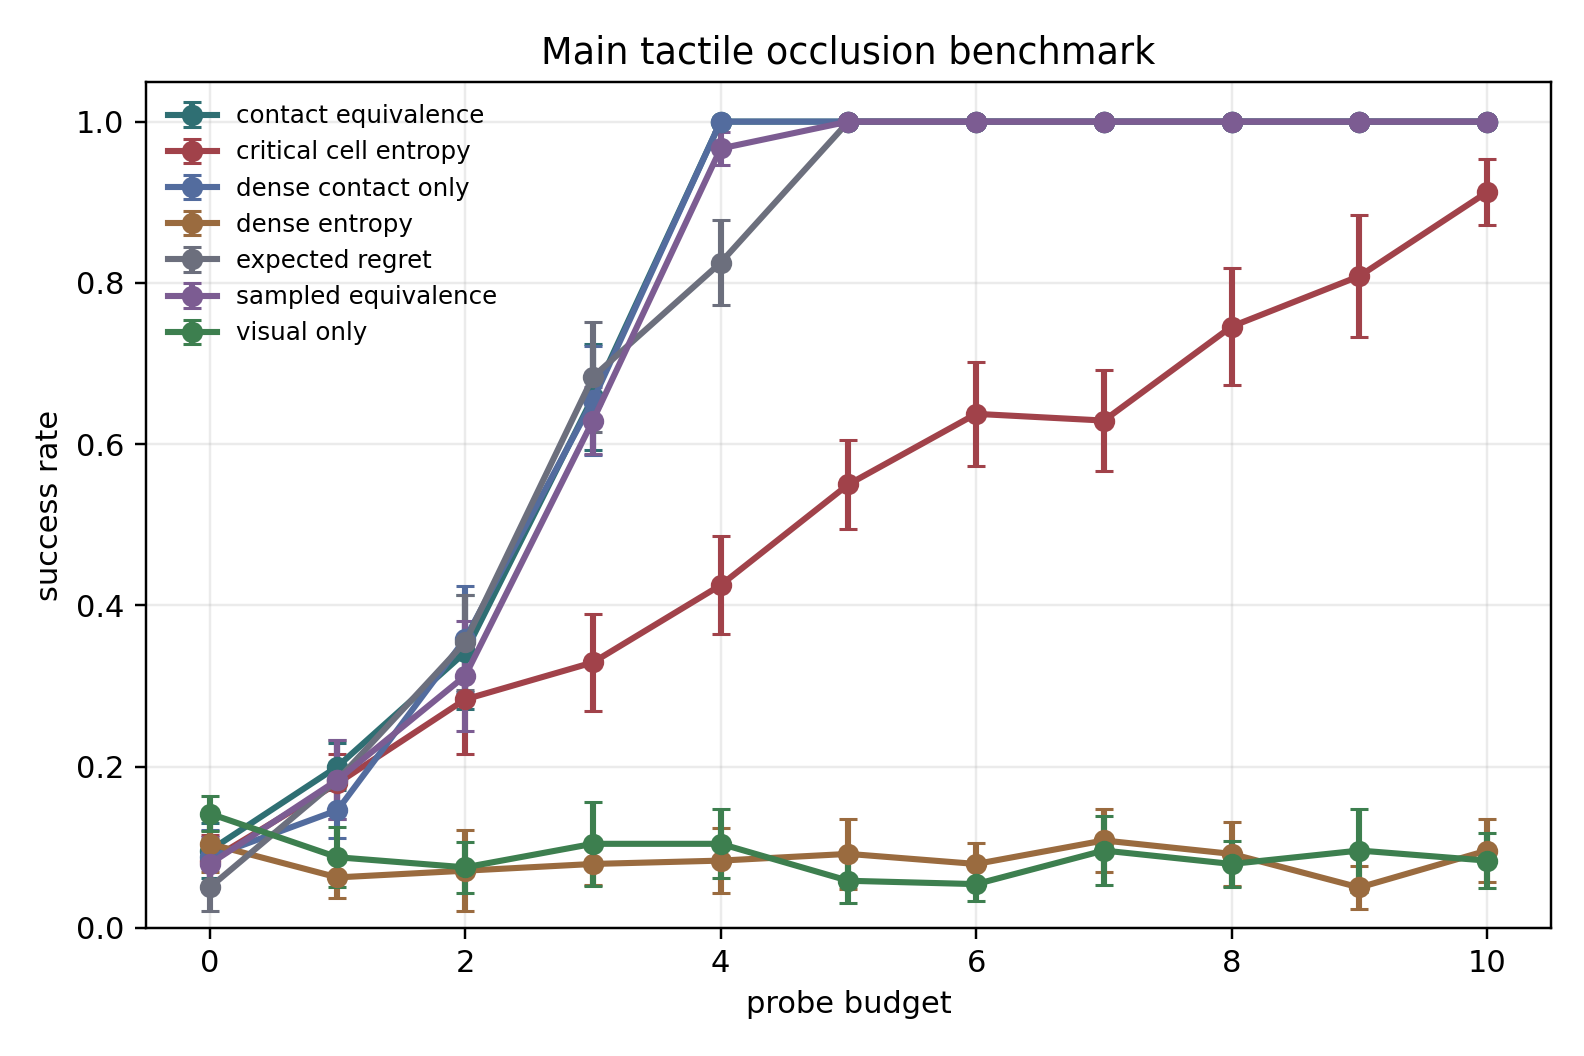
\includegraphics[width=0.80\linewidth]{figures/main_success_budget.png}
    \caption{Main success-vs-budget curves. Contact-equivalence and dense contact-only reach perfect success at budget four. Dense entropy over the full hidden state does not improve because it values decorative bits.}
    \label{fig:main}
\end{figure}

At budget four, contact-equivalence reaches 100.0\% success. Dense contact-only also reaches 100.0\%, confirming the boundary condition. Critical-cell entropy reaches 42.5\% because it asks lane-is-$i$ questions one at a time. Expected regret reaches 82.5\%, and sampled equivalence reaches 96.7\%, showing that approximate or regret-based contact probing can capture much of the benefit. Dense entropy reaches 8.3\%, essentially visual-only performance, because its first four probes are decorative.

Table~\ref{tab:allocation} makes the mechanism explicit. Dense entropy uses zero contact probes and four decorative probes at budget four. Contact-equivalence uses four contact probes and zero decorative probes, reducing posterior contact entropy to zero while leaving full hidden entropy high. This is the desired behavior: full geometry remains unknown, but the manipulation decision is resolved.

\begin{table}[t]
\centering
\caption{Budget-four posterior and probe allocation. Contact-equivalence leaves decorative geometry unresolved but removes contact ambiguity.}
\label{tab:allocation}
\resizebox{\linewidth}{!}{
\begin{tabular}{lrrrrr}
\toprule
Method & Success & Contact entropy & Full entropy & Contact probes & Decor probes \\
\midrule
Visual only & 0.104 & 3.585 & 67.585 & 0.000 & 0.000 \\
Dense entropy & 0.083 & 3.585 & 51.585 & 0.000 & 4.000 \\
Hybrid 50 & 0.100 & 3.585 & 51.585 & 0.000 & 4.000 \\
Critical-cell entropy & 0.425 & 1.962 & 65.962 & 4.000 & 0.000 \\
Expected regret & 0.825 & 0.317 & 64.317 & 4.000 & 0.000 \\
Sampled equivalence & 0.967 & 0.054 & 64.054 & 4.000 & 0.000 \\
Contact-equivalence & 1.000 & 0.000 & 64.000 & 4.000 & 0.000 \\
\bottomrule
\end{tabular}}
\end{table}

\begin{figure}[t]
    \centering
    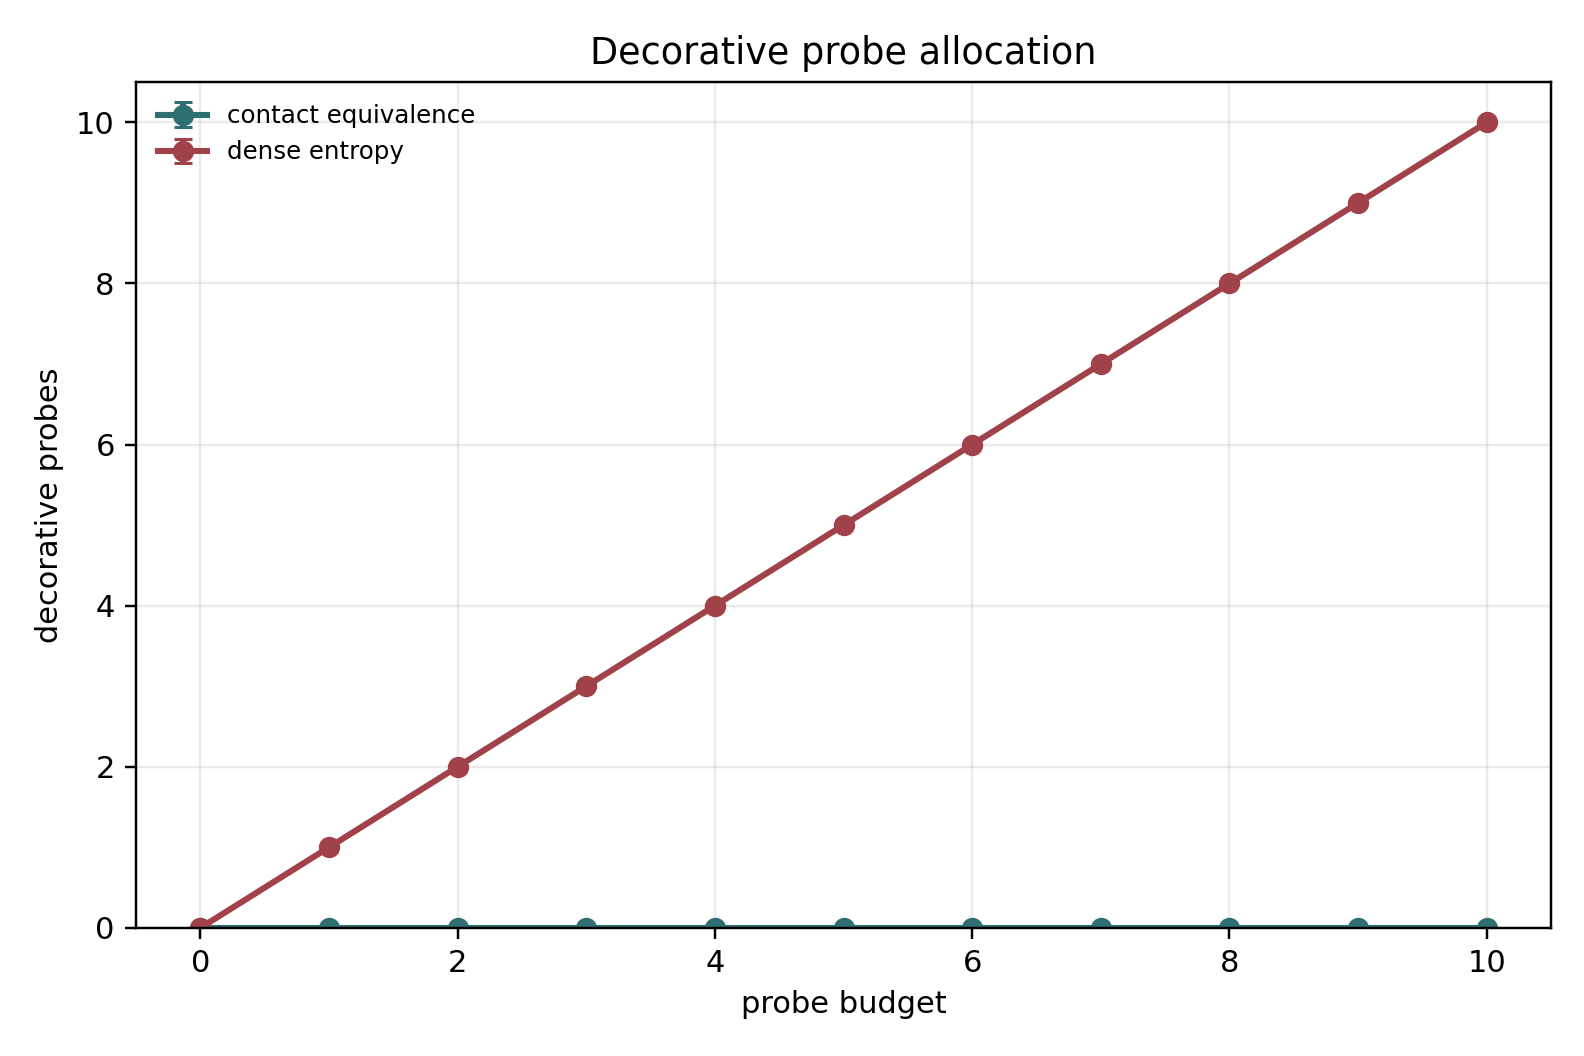
\includegraphics[width=0.72\linewidth]{figures/probe_allocation.png}
    \caption{Decorative probe allocation. Dense entropy spends budget on decorative bits; contact-equivalence spends budget on contact probes.}
    \label{fig:allocation}
\end{figure}

\section{Irrelevant Hidden-State Scaling}

The decorative-bit scaling suite varies how many visually hidden variables are irrelevant to contact. Table~\ref{tab:decor} reports budget-four success. With zero decorative bits, dense entropy and contact-equivalence both reach 100.0\%. With 16 or more decorative bits, dense entropy falls near visual-only, while contact-equivalence and dense contact-only remain at 100.0\%.

\begin{table}[t]
\centering
\caption{Budget-four success as irrelevant hidden variables increase. Dense entropy fails exactly when decorative hidden variables dominate full-state entropy.}
\label{tab:decor}
\resizebox{\linewidth}{!}{
\begin{tabular}{rrrrrr}
\toprule
Decor bits & Dense entropy & Hybrid 50 & Critical-cell & Expected regret & Contact-equivalence \\
\midrule
0 & 1.000 & 1.000 & 0.442 & 0.812 & 1.000 \\
16 & 0.075 & 0.083 & 0.438 & 0.850 & 1.000 \\
64 & 0.050 & 0.083 & 0.392 & 0.862 & 1.000 \\
128 & 0.083 & 0.075 & 0.425 & 0.858 & 1.000 \\
256 & 0.079 & 0.104 & 0.454 & 0.871 & 1.000 \\
\bottomrule
\end{tabular}}
\end{table}

\begin{figure}[t]
    \centering
    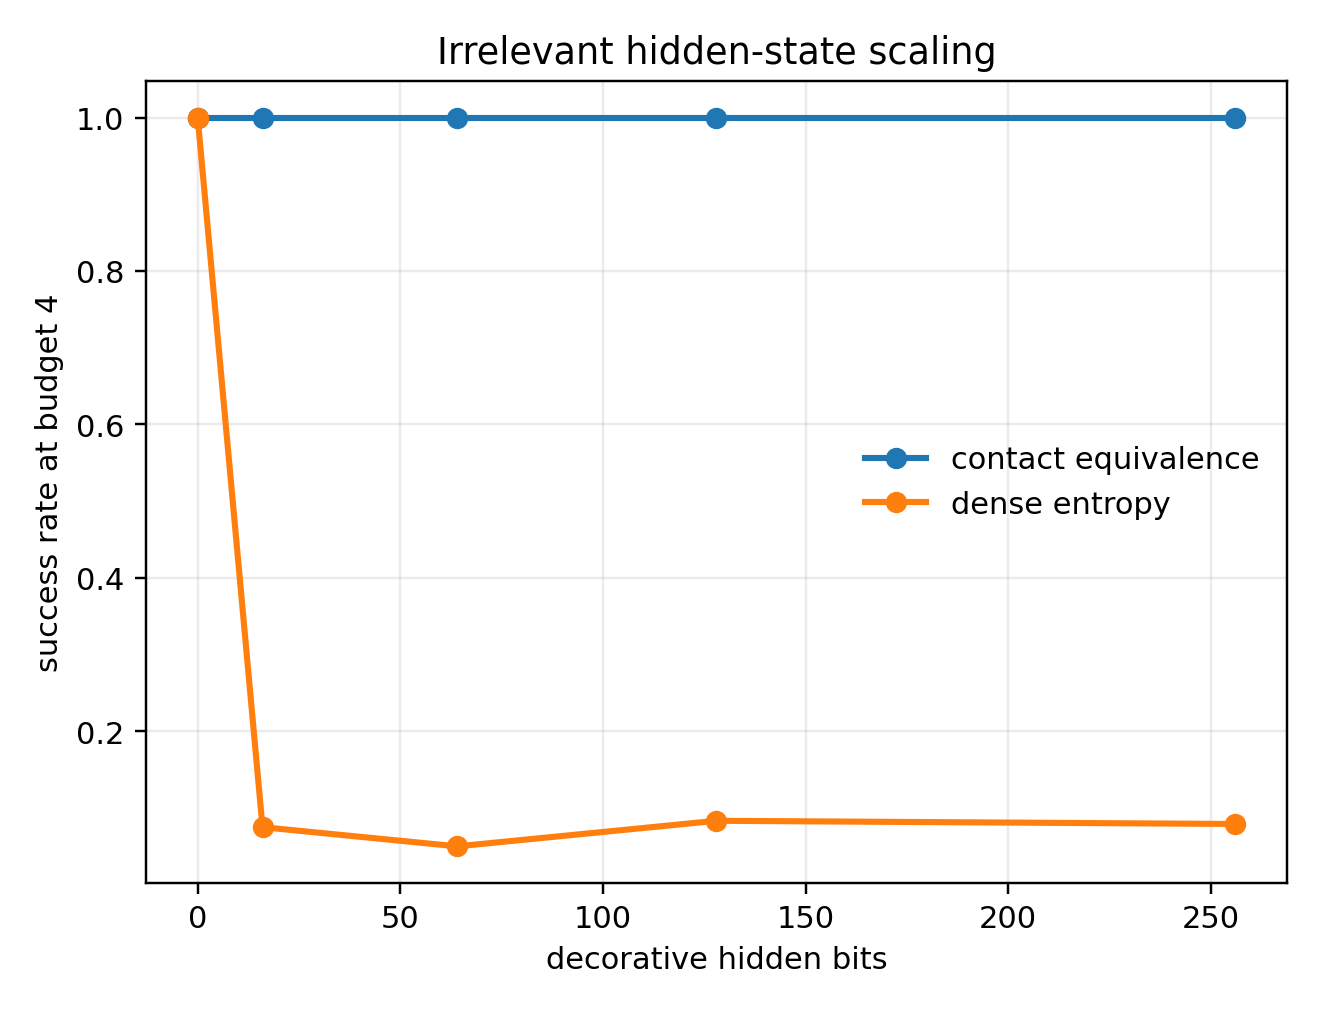
\includegraphics[width=0.70\linewidth]{figures/decor_scaling.png}
    \caption{Irrelevant hidden-state scaling. Dense entropy matches the quotient when no decorative bits exist, then fails once irrelevant hidden variables dominate entropy.}
    \label{fig:decor}
\end{figure}

This is the cleanest boundary result. Contact-equivalence is not better because entropy is bad. It is better because the dense state includes variables that do not affect the current manipulation. Once those variables are removed, dense entropy is again a good objective.

\section{Contact-Class Count Scaling}

The lane-scaling suite varies the number of hidden contact classes from 8 to 32. At budget six, exact contact-equivalence and dense contact-only remain at 100.0\%. Critical-cell entropy degrades from 88.8\% at 8 lanes to 21.2\% at 32 lanes because single-lane questions scale poorly. Expected regret remains strong through 16 lanes but drops to 67.1\% at 32 lanes. Sampled equivalence reaches 93.8\% at 32 lanes.

\begin{table}[t]
\centering
\caption{Budget-six success as hidden contact classes increase. Balanced quotient splits scale better than one-cell questions.}
\label{tab:lanes}
\resizebox{\linewidth}{!}{
\begin{tabular}{rrrrrr}
\toprule
Lanes & Dense entropy & Critical-cell & Expected regret & Sampled equivalence & Contact-equivalence \\
\midrule
8 & 0.133 & 0.888 & 1.000 & 1.000 & 1.000 \\
12 & 0.108 & 0.588 & 1.000 & 1.000 & 1.000 \\
16 & 0.054 & 0.425 & 1.000 & 1.000 & 1.000 \\
24 & 0.046 & 0.338 & 0.900 & 1.000 & 1.000 \\
32 & 0.021 & 0.212 & 0.671 & 0.938 & 1.000 \\
\bottomrule
\end{tabular}}
\end{table}

\begin{figure}[t]
    \centering
    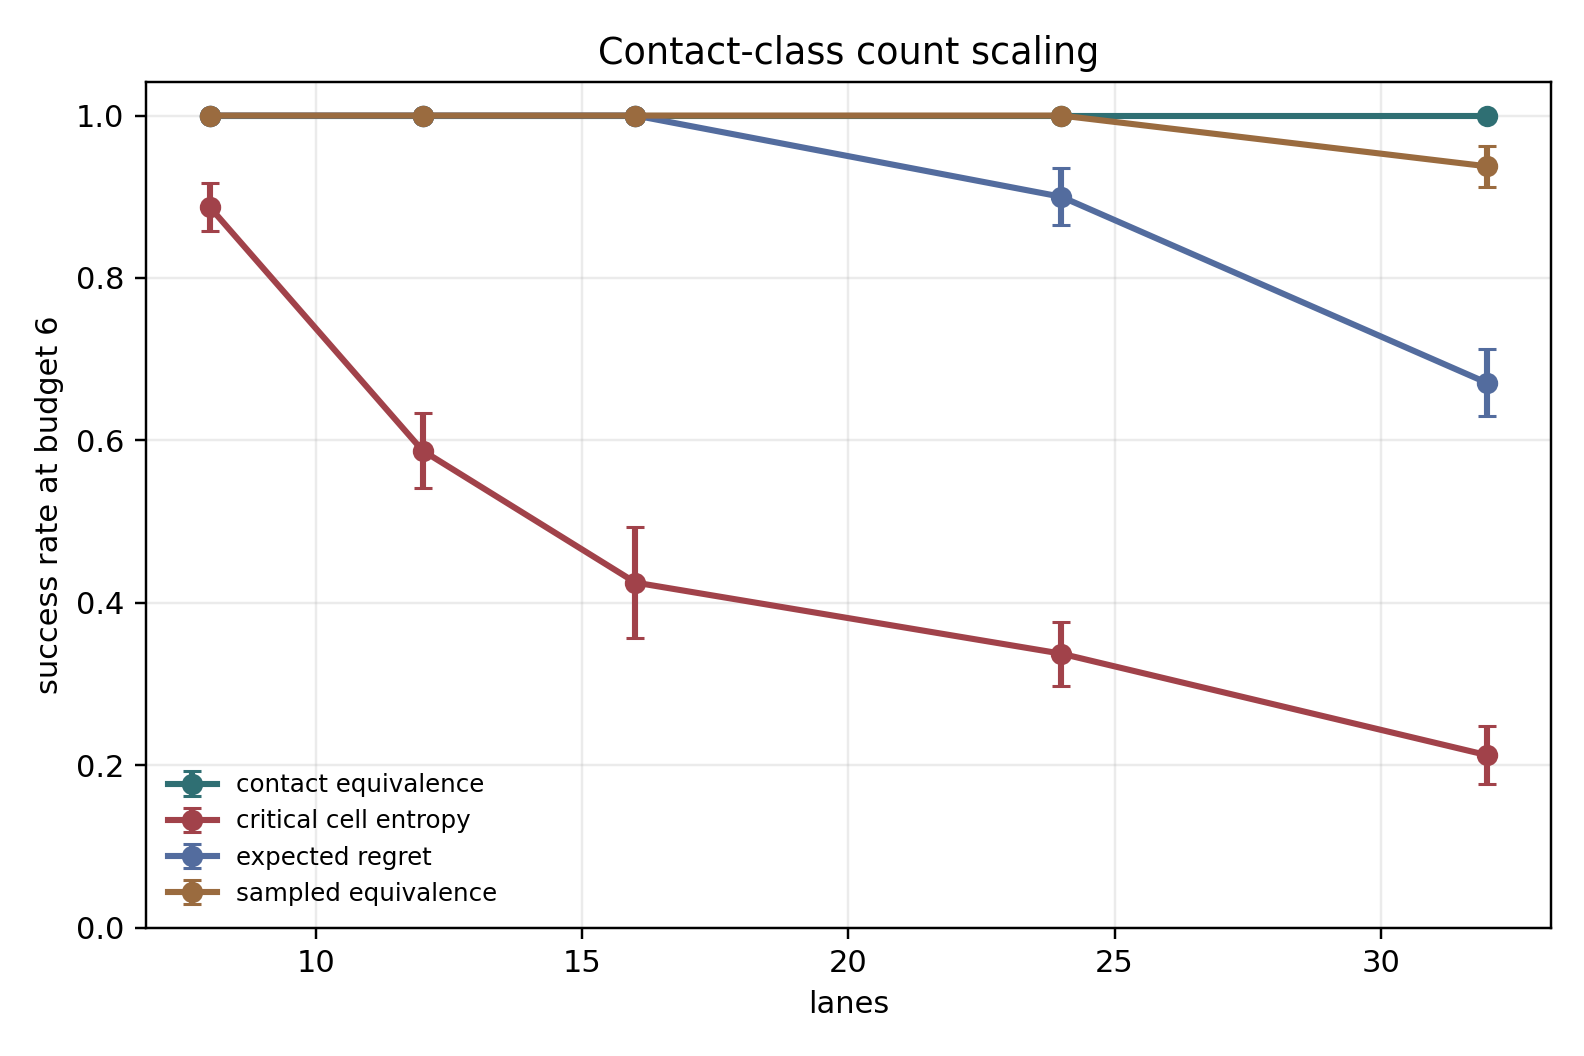
\includegraphics[width=0.78\linewidth]{figures/lane_scaling.png}
    \caption{Contact-class count scaling at budget six. Exact quotient splits remain strong; one-cell entropy scales poorly.}
    \label{fig:lanes}
\end{figure}

The result suggests that the useful probe primitive is not merely ``touch a contact cell.'' It is a tactile question that partitions the contact-outcome posterior. In real manipulation, such questions might be sweeps, guarded motions, or compliant exploratory actions.

\section{Tactile Noise Taxonomy}

The noise suite separates symmetric, false-positive, false-negative, and drift-like binary observation noise. Table~\ref{tab:noise} reports contact-equivalence success at budget four.

\begin{table}[t]
\centering
\caption{Contact-equivalence budget-four success under tactile noise modes. Symmetric and drift-like noise are most damaging.}
\label{tab:noise}
\begin{tabular}{lrrrrrr}
\toprule
Mode & 0\% & 2\% & 5\% & 10\% & 20\% & 30\% \\
\midrule
Symmetric & 1.000 & 0.912 & 0.821 & 0.675 & 0.442 & 0.208 \\
False positive & 1.000 & 0.954 & 0.933 & 0.858 & 0.683 & 0.600 \\
False negative & 1.000 & 0.967 & 0.904 & 0.858 & 0.712 & 0.529 \\
Drift-like & 1.000 & 0.917 & 0.833 & 0.675 & 0.358 & 0.254 \\
\bottomrule
\end{tabular}
\end{table}

\begin{figure}[t]
    \centering
    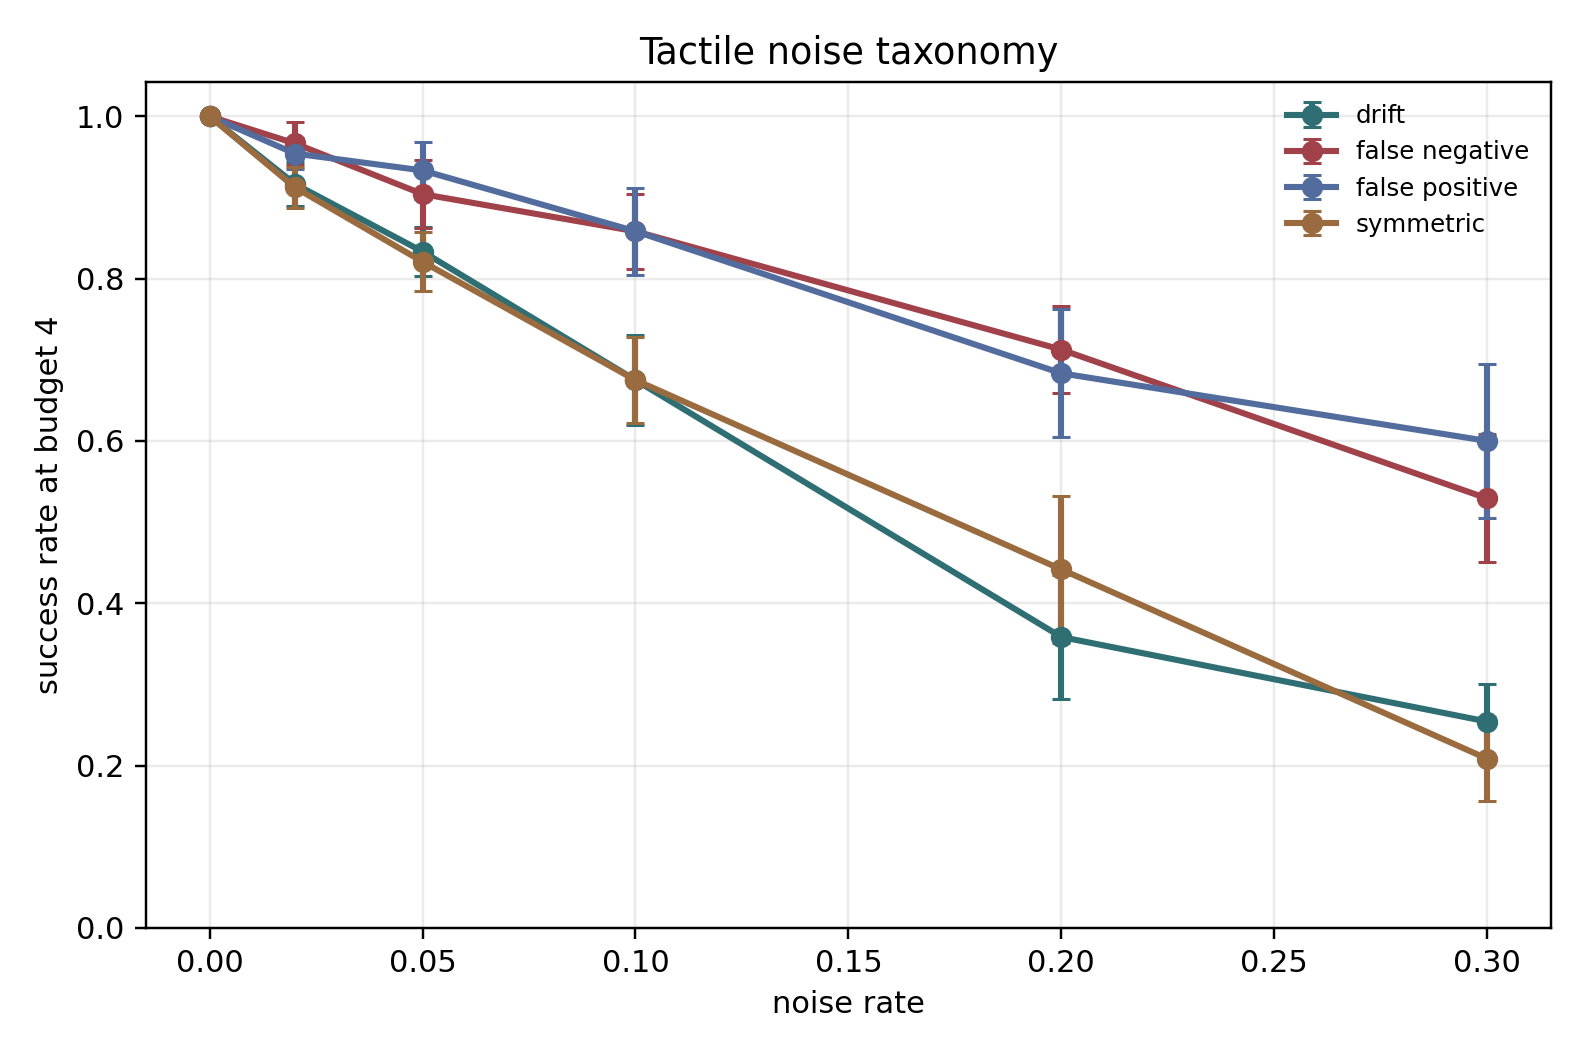
\includegraphics[width=0.78\linewidth]{figures/noise_taxonomy.png}
    \caption{Tactile noise taxonomy. Contact-equivalence degrades gracefully at low noise but fails under high symmetric or drift-like noise.}
    \label{fig:noise}
\end{figure}

At 20\% symmetric noise, success falls to 44.2\%. False-positive and false-negative modes are less damaging at the same nominal rate because they perturb only one side of the binary observation. Drift-like noise is severe because later probes become less reliable. This is a limitation, not a deployment claim. Real tactile calibration must be modeled before quotient reasoning can be trusted on hardware.

\section{Prior and Visual-Censoring Stress}

The prior-stress suite tests uniform, skewed, bimodal, and visually narrowed posteriors with 16 lanes. Table~\ref{tab:prior} reports budget-four success.

\begin{table}[t]
\centering
\caption{Budget-four success under prior and visual-censoring stress. Narrow visual ambiguity makes the task easy for all contact-aware methods; dense entropy remains distracted by decorative bits.}
\label{tab:prior}
\resizebox{\linewidth}{!}{
\begin{tabular}{lrrrrrr}
\toprule
Prior mode & Dense entropy & Critical-cell & Expected regret & Sampled equivalence & Dense contact-only & Contact-equivalence \\
\midrule
Uniform & 0.067 & 0.258 & 0.692 & 0.883 & 1.000 & 1.000 \\
Skewed & 0.204 & 0.750 & 0.821 & 0.929 & 0.958 & 0.958 \\
Bimodal & 0.162 & 0.538 & 0.829 & 0.879 & 0.904 & 0.904 \\
Visual narrow & 0.221 & 1.000 & 1.000 & 1.000 & 1.000 & 1.000 \\
\bottomrule
\end{tabular}}
\end{table}

\begin{figure}[t]
    \centering
    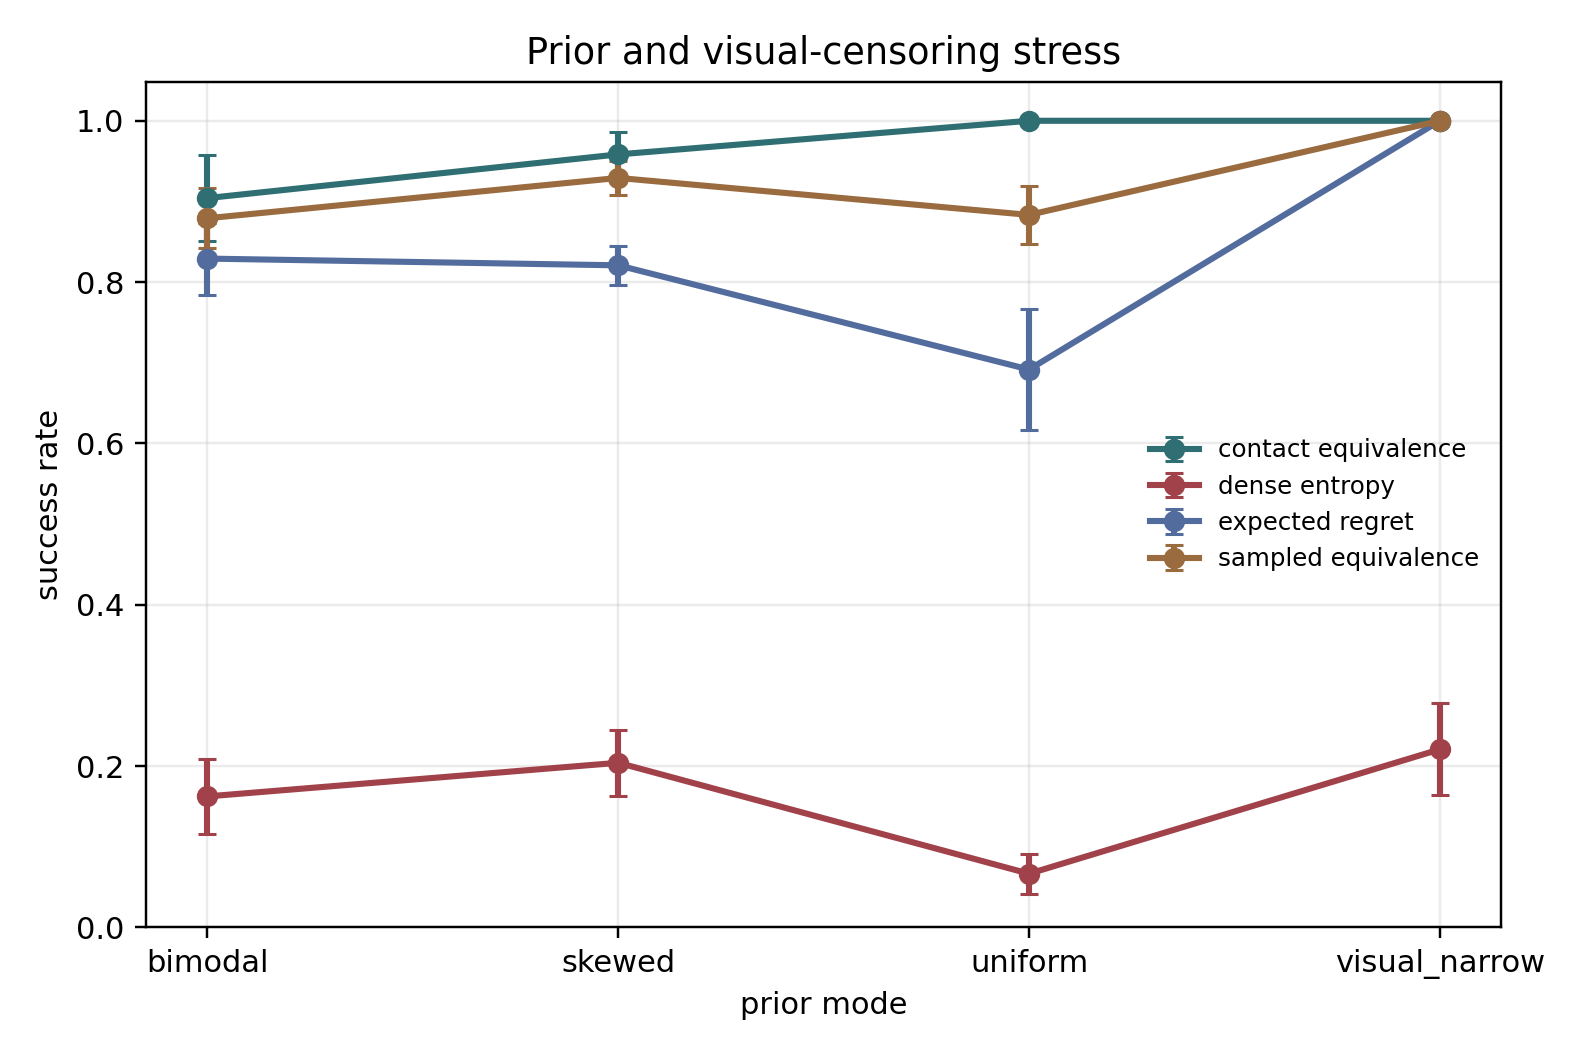
\includegraphics[width=0.78\linewidth]{figures/prior_stress.png}
    \caption{Prior and visual-censoring stress. Contact-aware objectives remain strong; dense entropy still values decorative bits when they are present.}
    \label{fig:prior}
\end{figure}

Skewed and bimodal priors reduce the maximum possible value of a balanced split because the posterior is no longer uniform over lanes. Contact-equivalence remains strong but no longer always reaches 100.0\% at budget four. This is another useful boundary: quotient probing is not magic; it is an information objective over whatever posterior vision leaves behind.

\section{Probe-Library Ablations}

Probe design matters. Table~\ref{tab:library} shows budget-four success under different libraries. With a mixed library, contact-equivalence reaches 100.0\%. With cells only, it drops to 40.4\%, similar to critical-cell entropy. With sweeps only, it reaches 68.8\%. With a contact-only library, dense entropy reaches 100.0\% because decorative distractors are removed.

\begin{table}[t]
\centering
\caption{Budget-four probe-library ablation. The representation needs useful contact-splitting probes; with cells only, equivalence loses its balanced-split advantage.}
\label{tab:library}
\begin{tabular}{lrrrr}
\toprule
Library & Dense entropy & Critical-cell & Expected regret & Contact-equivalence \\
\midrule
Mixed & 0.075 & 0.471 & 0.779 & 1.000 \\
Cells only & 0.075 & 0.471 & 0.433 & 0.404 \\
Sweeps only & 0.075 & 0.046 & 0.612 & 0.688 \\
Balanced only & 0.075 & 0.046 & 0.267 & 0.358 \\
Contact only & 1.000 & 0.471 & 0.779 & 1.000 \\
\bottomrule
\end{tabular}
\end{table}

\begin{figure}[t]
    \centering
    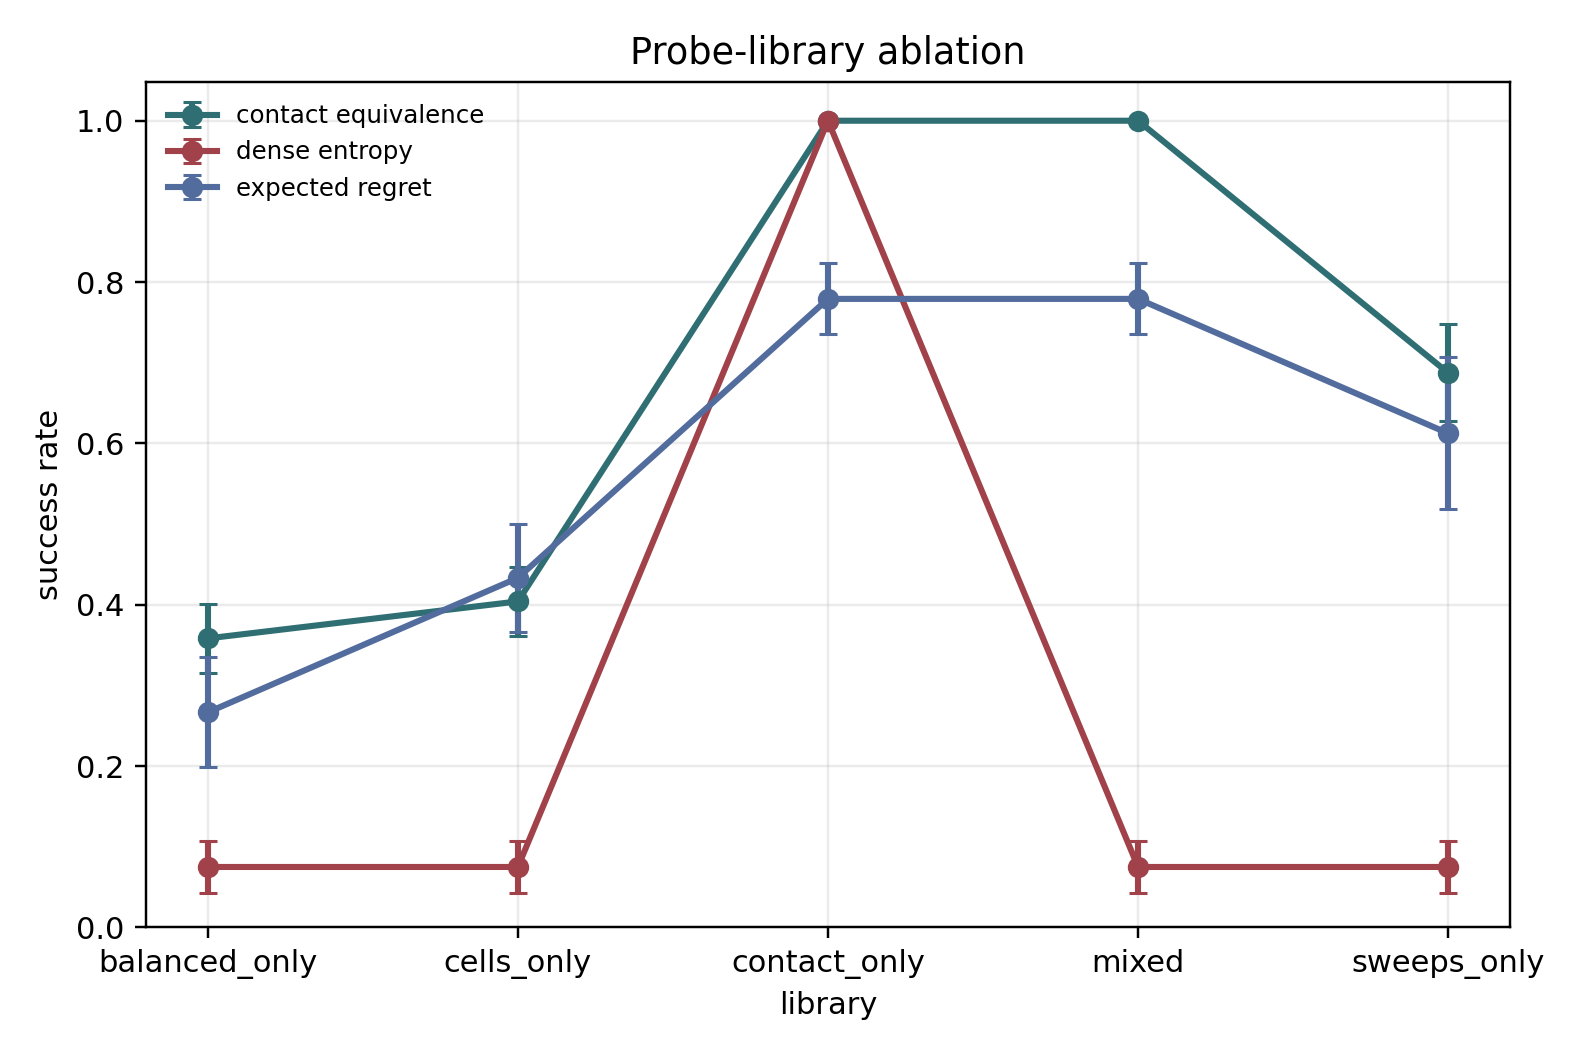
\includegraphics[width=0.78\linewidth]{figures/probe_library.png}
    \caption{Probe-library ablation. Contact-equivalence needs contact-splitting probes; dense entropy succeeds once the library is contact-only.}
    \label{fig:library}
\end{figure}

This suite prevents overclaiming. A quotient objective does not invent information. If the tactile action set cannot split the posterior effectively, performance is limited by the available questions.

\section{Boundary and Negative Controls}

The negative-control suite includes no-decor, oracle-filtered, decor-dominates, and cells-only-no-sweeps cases. Table~\ref{tab:negative} reports budget-four success.

\begin{table}[t]
\centering
\caption{Boundary and negative controls at budget four. Dense entropy succeeds when irrelevant hidden variables are removed; contact-equivalence suffers when the probe library lacks useful split probes.}
\label{tab:negative}
\resizebox{\linewidth}{!}{
\begin{tabular}{lrrrrrr}
\toprule
Case & Dense entropy & Dense contact-only & Critical-cell & Expected regret & Sampled equivalence & Contact-equivalence \\
\midrule
No decor & 1.000 & 1.000 & 0.412 & 0.838 & 0.979 & 1.000 \\
Oracle filtered & 1.000 & 1.000 & 0.438 & 0.838 & 0.983 & 1.000 \\
Decor dominates & 0.075 & 1.000 & 0.412 & 0.871 & 0.996 & 1.000 \\
Cells only, no sweeps & 0.067 & 0.350 & 0.417 & 0.421 & 0.475 & 0.433 \\
\bottomrule
\end{tabular}}
\end{table}

\begin{figure}[t]
    \centering
    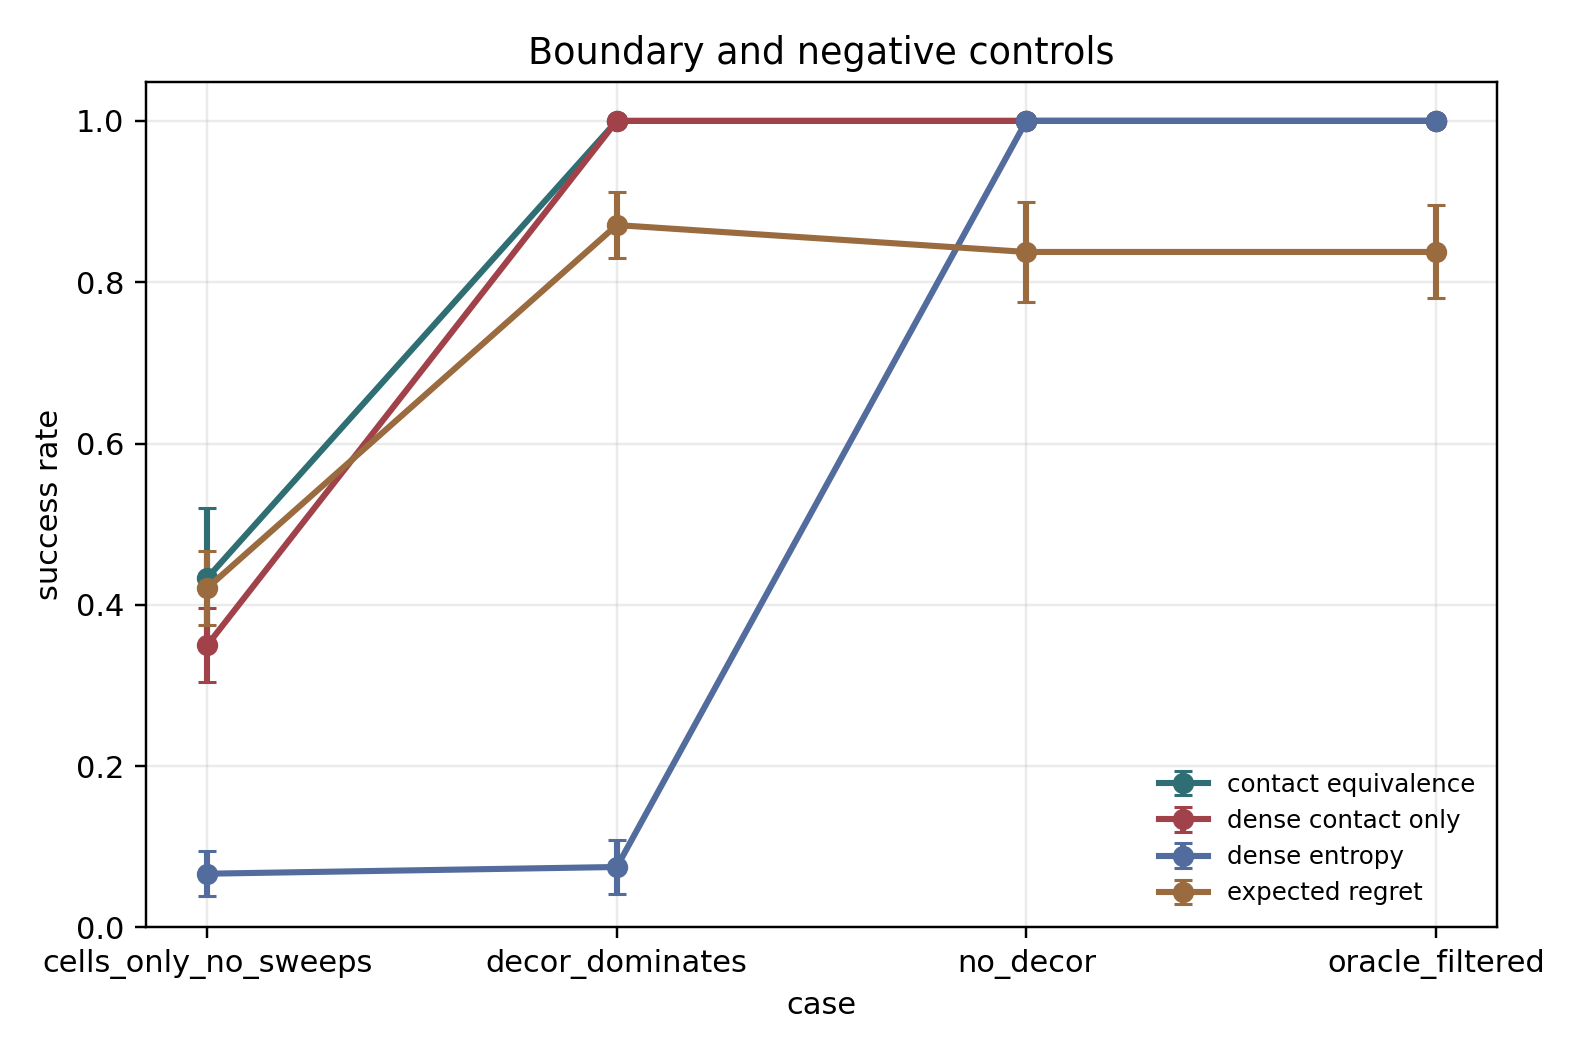
\includegraphics[width=0.78\linewidth]{figures/negative_controls.png}
    \caption{Boundary and negative controls. The dense objective is not inherently bad; it fails when irrelevant hidden variables dominate and succeeds when they are removed.}
    \label{fig:negative}
\end{figure}

These controls are central to the final claim. The paper should not be read as saying ``contact-equivalence always beats dense entropy.'' It says dense entropy over the wrong state can spend tactile budget on variables that cannot change the current manipulation decision.

\section{Discussion}

\paragraph{What the quotient buys.}
The quotient buys a decision-level representation. It tells the robot when it can stop exploring despite unresolved geometry, and it tells the active touch module which tactile questions matter. In the synthetic environment, it prevents decorative hidden variables from consuming the probe budget.

\paragraph{What the quotient does not buy.}
It does not make tactile observations reliable. It does not solve real 3D contact modeling. It does not create useful probes when the library lacks them. It does not dominate an oracle that has already filtered the hidden state to contact-relevant variables. It also does not remove the need for reconstruction when reconstruction is required for future actions.

\paragraph{Connection to planning.}
A planner can use contact-equivalence as a state abstraction. If all remaining hidden geometries in the belief induce the same outcome for the candidate action set, the planner can act without reconstructing further. If several equivalence classes remain, the planner should choose a tactile action that splits those classes. This is a natural interface between active perception and task-and-motion planning.

\section{Limitations}

The strongest limitation is that the environment is synthetic and stylized. Hidden geometry is a lane index plus decorative bits, not a mesh, articulated object, deformable object, or real contact surface. The result isolates a mechanism; it does not establish hardware readiness.

The second limitation is exact quotient maintenance. In real 3D, computing $C_a(g)$ for all plausible geometries may be expensive or impossible. The sampled-equivalence baseline is a small step toward approximation, but not a full solution.

The third limitation is tactile observation quality. The noise taxonomy shows that high noise and drift degrade performance. Real sensors have calibration drift, hysteresis, contact patch ambiguity, and dynamics not captured here.

The fourth limitation is that the probe library is hand-designed. Real robots need actions that produce informative contact splits without unsafe collisions. If only weak probes are available, the quotient objective cannot recover missing information.

The fifth limitation is that the task is single-step. Future actions may make currently irrelevant geometry relevant. A practical system should index equivalence by the current action set and update it as the plan changes.

\section{Conclusion}

Visual occlusion does not always require full tactile reconstruction. For manipulation, the robot often needs to know only which contact-outcome class the hidden geometry belongs to. Contact-equivalence reasoning makes that target explicit. The full-scale synthetic study shows when this quotient helps, when dense entropy is distracted, and when the advantage disappears. The next step is to approximate contact-equivalence partitions in realistic 3D manipulation with calibrated tactile observations and useful exploratory actions.

\section*{Reproducibility Statement}

The base simulator is in \texttt{experiments/tactile\_occlusion\_sim.py}. The expanded suite is generated by \texttt{experiments/run\_full\_scale\_tactile\_occlusion.py}. The final run was executed suite by suite with seed scale 10 and 24 trials per seed/condition. Outputs are compact CSVs under \texttt{results/full\_scale/}; figures are copied to \texttt{paper/figures/}. Raw per-trial trajectories are not stored.

\bibliographystyle{iclr2026_conference}
\bibliography{references}

\appendix

\section{Full-Scale Artifact Inventory}

\begin{table}[h]
\centering
\caption{Full-scale artifact inventory.}
\label{tab:inventory}
\resizebox{\linewidth}{!}{
\begin{tabular}{lrr}
\toprule
Suite file & Compact rows & Purpose \\
\midrule
\texttt{main\_budget.csv} & 1100 & Main success, entropy, and probe allocation by budget \\
\texttt{decor\_scaling.csv} & 1200 & Irrelevant hidden-state scaling \\
\texttt{lane\_scaling.csv} & 1500 & Contact-class count scaling \\
\texttt{noise\_taxonomy.csv} & 3600 & Symmetric, false-positive, false-negative, and drift noise \\
\texttt{prior\_stress.csv} & 960 & Prior and visual-censoring stress \\
\texttt{probe\_library.csv} & 800 & Probe-library ablations \\
\texttt{negative\_controls.csv} & 960 & Boundary and negative controls \\
\bottomrule
\end{tabular}
}
\end{table}

The total compact row count is 10,120. The total evaluated trial count, counting each row's trials, is 242,880. This count is not raw trajectory storage; it is the number of trial evaluations summarized into compact rows.

\section{Algorithmic Recipe}

The contact-equivalence active-touch loop is:

\begin{enumerate}
    \item Maintain a posterior over hidden geometries or over samples from that posterior.
    \item For the current action set, map each hidden geometry or sample to a contact-outcome tuple.
    \item Collapse geometries with identical outcome tuples into quotient cells.
    \item For each candidate tactile action, estimate expected reduction in quotient uncertainty or expected regret.
    \item Execute the best safe tactile action.
    \item Update the posterior and quotient.
    \item Stop when all remaining mass lies in one decision-equivalent class, or when the expected value of information is below action cost.
\end{enumerate}

The dense reconstruction loop differs only in step 4: it values reduction in full hidden geometry entropy. That one substitution is enough to produce the failure mode in the benchmark.

\section{Additional Formal Notes}

\begin{proposition}[Dense distraction by irrelevant variables]
Suppose the hidden state factors as $(Q,D)$, where $Q$ is the contact-equivalence class and $D$ is independent decorative geometry. If there exists a decorative probe revealing $k$ bits of $D$ and every available contact probe has dense information gain less than $k$, then greedy dense information gain selects the decorative probe even though it has zero information gain about $Q$.
\end{proposition}

\begin{proof}
The decorative probe reduces $H(D)$ by $k$ bits and does not change $H(Q)$. Since $Q$ and $D$ are independent, it reduces full entropy $H(Q,D)$ by $k$. By assumption, every contact probe has smaller dense information gain. Greedy dense information gain therefore selects the decorative probe. Its quotient gain is zero because the posterior over $Q$ is unchanged.
\end{proof}

\begin{proposition}[Boundary agreement]
If the hidden state contains only contact-relevant variables, or if the probe library excludes probes that affect only contact-irrelevant variables, then dense entropy and contact-equivalence can rank probes identically when the contact map is one-to-one on the remaining hidden state.
\end{proposition}

\begin{proof}
When the contact map is one-to-one on the remaining hidden state, the quotient variable $Q_A(G)$ is equivalent to $G$ up to relabeling. Entropy over $G$ and entropy over $Q_A(G)$ therefore differ only by the relabeling, and any probe's expected reduction is the same under both objectives.
\end{proof}

These propositions explain the main and boundary controls. Dense entropy is distracted when decorative bits exist. It agrees with contact-equivalence when decorative bits are removed or filtered.

\section{Noise Interpretation}

The noise taxonomy separates observation errors that are often conflated in synthetic tactile work. Symmetric noise flips both positive and negative contact answers. False-positive noise makes a probe report contact membership when the true lane is outside the subset. False-negative noise misses true membership. Drift-like noise increases effective error as probing proceeds.

At 20\% nominal rate, contact-equivalence success is 44.2\% under symmetric noise, 68.3\% under false-positive noise, 71.2\% under false-negative noise, and 35.8\% under drift-like noise. The ordering depends on the sweep structure and posterior update rule; it should not be assumed universal. The important point is that tactile calibration is a first-order part of the method.

\section{Reviewer-Facing Boundaries}

\paragraph{This is not just active touch.}
The robot is active, but the novelty is the quotient variable. Dense entropy, cell entropy, expected regret, and contact-equivalence all use active touch but choose different probes.

\paragraph{This is not anti-reconstruction.}
Reconstruction is appropriate when future decisions require the reconstructed geometry. The paper argues only that reconstruction is too fine-grained for a current contact decision when many hidden differences are decision-equivalent.

\paragraph{The dense contact-only control is not a threat.}
It is the boundary. It shows that once the state is filtered to contact-relevant variables, dense entropy can agree with the quotient. The contribution is knowing not to include irrelevant hidden variables in the objective for the current manipulation.

\paragraph{The simulator is stylized.}
Yes. The stylization isolates the hidden assumption. A realistic follow-up should replace lanes with contact outcome maps over 3D shape samples and replace binary sweeps with safe tactile exploration primitives.

\section{Path to Realistic Validation}

A realistic benchmark should include a set of visually ambiguous objects whose hidden shape variations are partly contact-relevant and partly irrelevant. For each object, the benchmark should define a current action set and contact-outcome labels generated by simulation or controlled hardware trials. Tactile actions should include local presses, guarded sweeps, and compliant insertions. The key metric should be manipulation decision accuracy as a function of tactile budget, not reconstruction Chamfer distance alone.

The benchmark should include oracle-filtered controls. If a method has already been handed the contact-relevant variables, dense entropy should perform well. The interesting question is whether a robot can avoid spending touches on hidden variables that are visually uncertain but irrelevant to the next manipulation.

\section{Claim Checklist}

Supported:
\begin{itemize}
    \item Dense hidden-state entropy can be distracted by manipulation-irrelevant hidden variables.
    \item Contact-equivalence probing resolves the synthetic hidden-lane task with fewer probes than dense entropy and critical-cell entropy.
    \item Dense entropy matches contact-equivalence when decorative variables are removed or the library is contact-only.
    \item Noise, priors, and probe-library limits materially affect performance.
\end{itemize}

Not supported:
\begin{itemize}
    \item Real-robot tactile deployment.
    \item Exact quotient maintenance over high-dimensional 3D geometry.
    \item Robustness to calibration drift beyond the synthetic taxonomy.
    \item Superiority over learned systems that already identify contact-relevant variables.
    \item Universal usefulness of contact-equivalence for future action sets whose relevant contacts may change.
\end{itemize}

\clearpage
\section{Suite Protocol Details}

This appendix gives the exact interpretation of each full-scale suite. The purpose is to make the result auditable and to prevent a single headline number from carrying more meaning than it should.

\paragraph{Main budget suite.}
The main suite uses 12 hidden lanes, 64 decorative bits, a uniform visual posterior, a mixed probe library, and noiseless tactile observations. It records budgets from 0 to 10. This suite is the closest successor to the base experiment. It tests whether different objectives spend the same probe budget on contact-relevant or contact-irrelevant variables. The central readout is budget four because four balanced sweeps are sufficient to identify one of 12 lanes in the mixed library. The dense objective fails not because it lacks tactile access, but because decorative probes each remove several bits of dense entropy and therefore dominate early greedy choices.

\paragraph{Decorative scaling suite.}
The decorative scaling suite holds the contact problem fixed and varies irrelevant hidden bits. The result shows a threshold behavior. With no decorative bits, dense entropy is not distracted and reaches perfect success at budget four. With 16 or more decorative bits, dense entropy selects decorative probes first and remains near chance. This is the cleanest evidence that the state variable, not the sensor, is the problem. A reconstruction objective over the wrong hidden state can optimize precisely and still be irrelevant to manipulation.

\paragraph{Lane scaling suite.}
The lane scaling suite varies the number of hidden contact classes. It distinguishes balanced contact splits from one-cell probes. Critical-cell entropy can eventually identify the lane, but its efficiency declines as the number of lanes grows. Contact-equivalence remains strong because the mixed library includes sweep probes that split the posterior. Expected-regret and sampled-equivalence are intermediate: they usually choose useful contact probes but can be less stable under many lanes and finite samples.

\paragraph{Noise taxonomy suite.}
The noise suite is not a real tactile model. It is a controlled way to separate failure modes. Symmetric noise flips both positive and negative answers. False-positive noise makes a subset probe report membership too often. False-negative noise misses true membership. Drift-like noise represents later probes becoming less reliable. The main lesson is that quotient reasoning depends on tactile calibration. If the observation model is wrong, quotient updates can become overconfident.

\paragraph{Prior stress suite.}
The prior suite changes what vision leaves behind. Uniform priors are hardest for single-cell probing. Skewed priors make visual-only and critical-cell methods stronger because the posterior already favors some lanes. Bimodal priors make balanced splits less perfect because the posterior mass is clustered. Visual-narrow priors are easy because vision has already reduced the contact ambiguity. This suite matters because the quotient objective operates on the posterior supplied by vision, not on an abstract uniform state.

\paragraph{Probe-library suite.}
The library suite asks whether the method has useful tactile questions. Mixed probes include decorative probes, single-lane probes, and sweeps. Cells-only removes sweep structure; contact-equivalence then loses its balanced split advantage. Sweeps-only removes single-lane tests and can still work, but not always perfectly at small budgets. Contact-only removes decorative probes; dense entropy then becomes a strong contact objective. This prevents a false claim that contact-equivalence is independent of action design.

\paragraph{Boundary and negative controls.}
The negative controls are really boundary controls. The no-decor and oracle-filtered cases show dense entropy matching contact-equivalence. The decor-dominates case shows the full failure mode. The cells-only-no-sweeps case shows that the quotient objective cannot overcome a weak probe library. Together these controls define where the representation helps and where it does not.

\section{Data Schema and Compact Artifacts}

The runner writes one row per suite, seed, method, budget, and condition. Common columns include \texttt{suite}, \texttt{seed}, \texttt{method}, \texttt{budget}, \texttt{trials}, \texttt{lanes}, \texttt{decor\_bits}, \texttt{library}, \texttt{noise\_mode}, \texttt{noise\_rate}, \texttt{prior\_mode}, \texttt{success\_rate}, \texttt{mean\_regret}, \texttt{posterior\_contact\_entropy}, \texttt{posterior\_full\_entropy}, \texttt{contact\_probes}, and \texttt{decor\_probes}. Suite-specific columns include \texttt{decor\_setting}, \texttt{lane\_setting}, and \texttt{case}.

\begin{table}[h]
\centering
\caption{Compact artifact schema. The first column gives the suite name rather than the full filename to avoid formatting artifacts; the CSV files use the corresponding suite names under \texttt{results/full\_scale/}.}
\label{tab:schema}
\resizebox{\linewidth}{!}{
\begin{tabular}{p{0.22\linewidth}p{0.34\linewidth}p{0.36\linewidth}}
\toprule
Suite & Key condition columns & Primary audit question \\
\midrule
Main budget & \texttt{budget}, \texttt{method} & Does contact-equivalence spend tactile budget on contact classes rather than decorative state? \\
Decor scaling & \texttt{decor\_bits}, \texttt{budget} & When do irrelevant hidden variables distract dense entropy? \\
Lane scaling & \texttt{lanes}, \texttt{budget} & How does one-cell probing scale compared with balanced quotient splits? \\
Noise taxonomy & \texttt{noise\_mode}, \texttt{noise\_rate} & Which tactile observation errors degrade quotient updates? \\
Prior stress & \texttt{prior\_mode} & How does the visual posterior shape change active touch value? \\
Probe library & \texttt{library} & Does the action set contain useful contact-splitting probes? \\
Negative controls & \texttt{case} & Does the claimed advantage disappear at the right boundaries? \\
\bottomrule
\end{tabular}}
\end{table}

The compact schema is deliberate. Raw trajectories are easy to regenerate but expensive to store and inspect. The scientific claims in this paper are aggregate claims about success, entropy, regret, and probe allocation under deterministic configurations. Compact rows retain the information needed to audit those claims while keeping the repository small.

\section{Baseline Failure Taxonomy}

Each baseline fails for a different reason.

\paragraph{Visual only.}
Visual only fails because the visual observation censors the lane. Under a uniform posterior over 12 lanes, visual success is near chance. When the prior is skewed or visually narrowed, visual-only performance would improve, but the robot still has unresolved contact ambiguity unless the posterior is already concentrated.

\paragraph{Dense entropy.}
Dense entropy fails when irrelevant hidden variables dominate the full state. It behaves exactly as designed: it removes many bits of uncertainty. The problem is that those bits are decorative. This is a representation failure, not an optimization failure.

\paragraph{Hybrid objectives.}
Hybrid dense/contact objectives can also fail when dense entropy receives enough weight that decorative probes still dominate early decisions. In the main budget-four table, hybrid 25 and hybrid 50 both spend all four probes on decorative bits. This shows that simply adding a small task-aware term may not be enough when dense irrelevant entropy is large.

\paragraph{Critical-cell entropy.}
Critical-cell entropy asks relevant questions but inefficient ones. A lane-is-$i$ probe can eliminate or confirm one lane. Balanced sweeps can split the posterior more evenly. This is why critical-cell entropy improves steadily with budget but is far below contact-equivalence at budget four.

\paragraph{Expected regret.}
Expected-regret probing is a strong decision-aware baseline. It reaches 82.5\% at budget four and 100.0\% by budget five in the main suite. Its weakness appears in larger lane counts and some library constraints, where a purely myopic regret objective can choose less balanced questions than quotient entropy.

\paragraph{Sampled equivalence.}
Sampled equivalence approximates the quotient with posterior samples. It reaches 96.7\% at budget four in the main suite and remains strong in lane scaling. Its residual failures are a useful proxy for approximate quotient maintenance in realistic settings: approximation can work, but finite samples and noisy posteriors matter.

\section{Additional Result Interpretation}

\paragraph{Why contact entropy can be zero while full entropy is high.}
At budget four, contact-equivalence has posterior contact entropy 0.000 and posterior full entropy 64.000. This is not a contradiction. The four probes identify the lane, leaving all 64 decorative bits unknown. The manipulation action is resolved because decorative bits do not affect the contact outcome. This is the central idea of the paper in one number.

\paragraph{Why dense entropy can reduce full entropy without improving success.}
Dense entropy reduces full entropy from 67.585 to 51.585 at budget four. It has made progress on reconstruction. But contact entropy remains 3.585, exactly the unresolved lane entropy. Manipulation success remains near chance. This is why reconstruction metrics alone can be misleading for manipulation under occlusion.

\paragraph{Why no-decor controls matter.}
With zero decorative bits, dense entropy reaches 100.0\% at budget four. This prevents an unfair straw baseline. Dense entropy is not inherently poor; dense entropy over a state containing irrelevant hidden variables is the problem. The no-decor and contact-only controls therefore strengthen the paper by narrowing the mechanism.

\paragraph{Why cells-only hurts contact-equivalence.}
Contact-equivalence is an objective over quotient classes, not a guarantee that the action set can split them efficiently. If the library contains only single-lane probes, the best quotient objective still has to ask narrow questions. The cells-only-no-sweeps negative control reduces contact-equivalence to 43.3\% at budget four, close to critical-cell behavior.

\section{Approximation Strategies for Real Geometry}

Exact equivalence classes over 3D hidden geometry are unlikely to be enumerated in a real robot. The representation can still guide approximations.

\paragraph{Sampled quotient.}
Maintain particles or shape samples from a visual posterior. For each candidate action, simulate or approximate the contact outcome for each sample. Group samples by outcome tuple. Choose tactile probes that split sample groups. The sampled-equivalence baseline in this paper is a small version of this idea.

\paragraph{Learned contact-outcome maps.}
Instead of reconstructing full geometry, train a model to predict contact outcomes for candidate actions from partial geometry and tactile history. The quotient then lives in the model's outcome space. This would be a learned approximation to $C_a(g)$ rather than a hand-coded lane map.

\paragraph{Hashing and abstraction.}
For high-dimensional geometry, exact equality of contact outcomes may be too brittle. A robot could hash outcomes into approximate classes: collision/no collision, slip/no slip, insertion depth bins, or stable/unstable grasp pockets. The abstraction should be chosen by downstream decision loss, not by geometric fidelity alone.

\paragraph{Planner-coupled quotienting.}
A task-and-motion planner can propose the current action set $A$. The quotient is then indexed by that action set. When the plan changes, the equivalence relation changes. This avoids computing a universal object partition and keeps tactile reasoning local to the current decision.

\section{Hardware Validation Design}

A hardware validation should preserve the quotient question rather than merely show a tactile robot succeeding. A useful design would include objects with hidden contact-relevant and contact-irrelevant variations. For example, an insertion fixture could hide the true channel while also hiding decorative backside features. A transparent or reflective object could hide both a contact lip and irrelevant surface texture. A drawer-like object could vary the latch pocket while also varying unrelated interior geometry.

The protocol should log:
\begin{itemize}
    \item visual posterior or ambiguity set;
    \item candidate manipulation actions;
    \item tactile actions and their costs;
    \item contact-outcome labels or downstream success;
    \item reconstruction metrics, if reconstruction is performed;
    \item decision metrics such as success, regret, and number of touches.
\end{itemize}

The key comparison should be between reconstructing all hidden geometry and resolving the contact-equivalence class for the current action. A hardware benchmark that reports only final task success would be insufficient because several methods might succeed after many touches. The relevant question is whether the robot spends touches on decision-relevant ambiguity.

\section{Extended Literature Boundary}

The broad tactile literature makes many possible claims non-novel. Sensor papers improve observation fidelity. Reconstruction papers recover shape. Pose papers localize objects or contacts. Active haptic papers choose informative touches. Visuo-tactile policy papers learn multimodal control. This paper is narrower than all of those: it asks what hidden variable active touch should reduce when the manipulation decision is already specified.

\begin{table}[h]
\centering
\caption{Literature-boundary map.}
\label{tab:litboundary}
\resizebox{\linewidth}{!}{
\begin{tabular}{p{0.26\linewidth}p{0.30\linewidth}p{0.34\linewidth}}
\toprule
Area & Makes less novel & What remains open for this paper \\
\midrule
Tactile sensing & Measuring local contact accurately & Which hidden variables should be ignored for a decision \\
Shape reconstruction & Recovering hidden surfaces from touch & Stopping before reconstruction when contact outcome is known \\
Pose and tracking & Estimating object/contact state & Quotienting geometries that differ but have same action outcome \\
Active haptics & Choosing informative touch actions & Choosing information over contact-equivalence rather than dense state \\
Visuo-tactile policies & Learning end-to-end behavior & Auditable target variable for hidden geometry under occlusion \\
Task planning & Evaluating actions and contacts & Passing quotient uncertainty to the planner instead of dense geometry alone \\
\bottomrule
\end{tabular}}
\end{table}

\section{Compute and Memory Notes}

The full-scale runner was written after the base simulator proved too slow to force-regenerate in a single command window. The new runner records compact rows and reuses each trajectory across budgets. It runs suites sequentially and writes one CSV per suite. The final artifact counts 10,120 rows and 242,880 evaluated trials counted across rows. This is enough to stabilize the major synthetic effects while keeping memory use small.

The runner intentionally does not save raw touch sequences. Raw sequences would be useful for debugging individual trials but unnecessary for the aggregate claims. If a future hardware or 3D simulator produces expensive raw data, the same pattern should hold: save compact summaries for paper claims, and save raw traces only for selected diagnostic cases.

\section{Reproducibility Commands}

The final full-scale run can be reproduced suite by suite:

\begin{verbatim}
python experiments/run_full_scale_tactile_occlusion.py
  --suite main --seed-scale 10 --trials 24 --fresh
python experiments/run_full_scale_tactile_occlusion.py
  --suite decor --seed-scale 10 --trials 24
python experiments/run_full_scale_tactile_occlusion.py
  --suite lanes --seed-scale 10 --trials 24
python experiments/run_full_scale_tactile_occlusion.py
  --suite noise --seed-scale 10 --trials 24
python experiments/run_full_scale_tactile_occlusion.py
  --suite prior --seed-scale 10 --trials 24
python experiments/run_full_scale_tactile_occlusion.py
  --suite library --seed-scale 10 --trials 24
python experiments/run_full_scale_tactile_occlusion.py
  --suite negative --seed-scale 10 --trials 24
python experiments/run_full_scale_tactile_occlusion.py
  --suite summarize --seed-scale 10
\end{verbatim}

The manuscript can then be rebuilt from \texttt{paper/} with \texttt{pdflatex}, \texttt{bibtex}, and two further \texttt{pdflatex} passes. The rebuilt document should contain the full-scale figures and the 10,120-row scale claim.

\section{Ethical and Practical Notes}

This paper is synthetic and does not introduce an immediate deployment risk. The practical lesson is still safety-relevant: a robot should not spend physical contact budget on tactile actions that cannot affect the current manipulation decision. In cluttered or human-facing environments, unnecessary touch can damage objects or create unsafe contacts. A decision-level information target can reduce unnecessary exploration, provided the contact-outcome model and tactile observations are trustworthy.

The same idea can also prevent overconfidence. If the robot has not resolved the contact-equivalence class, it should not act as if a dense reconstruction prior has solved the manipulation problem. Conversely, if the class is resolved but geometry remains unknown, the robot should know that further reconstruction is optional for the current action but may be needed for future actions.

\section{Bayesian Update Details}

The lane simulator is small enough that the posterior can be updated exactly. Let $q\in\{1,\ldots,L\}$ be the hidden contact class. A lane probe asks whether $q=i$. A sweep probe asks whether $q\in S$ for a subset $S$. For a binary observation $z\in\{0,1\}$ with false-positive rate $\alpha$ and false-negative rate $\beta$, the likelihood is
\[
    p(z=1\mid q,t)=
    \begin{cases}
    1-\beta, & q\in S_t,\\
    \alpha, & q\notin S_t,
    \end{cases}
\]
where $S_t$ is either a singleton lane or a sweep subset. The posterior update is
\[
    b_{t+1}(q)=
    \frac{b_t(q)p(z\mid q,t)}
    {\sum_{q'} b_t(q')p(z\mid q',t)}.
\]
Dense decorative probes update only decorative variables. In the compact implementation, decorative variables are counted by how many hidden bits have been revealed; they do not appear in the contact posterior because they are independent of $q$ and irrelevant to the contact outcome.

\paragraph{Expected quotient information.}
For a candidate probe $t$, exact contact-equivalence information gain is
\[
    H(b_t(q)) -
    \sum_{z\in\{0,1\}} p(z\mid b_t,t)H(b_t(q\mid z,t)).
\]
This is the same algebra as ordinary information gain, but the entropy is over the contact quotient rather than over all hidden variables. In the lane benchmark the quotient variable is the lane itself. In a richer problem, many geometries can map to the same contact outcome, and entropy would be computed after grouping those geometries.

\paragraph{Expected regret.}
The expected-regret baseline uses the same posterior but optimizes a different criterion. Before probing, its decision regret surrogate is $1-\max_q b_t(q)$. After a candidate observation, it computes the expected value of the same surrogate under the updated posterior. This objective is very strong in the main benchmark because any probe that quickly creates a dominant lane is valuable. It is less directly tied to balanced partitioning, which explains why it can lag contact-equivalence under larger lane counts or weaker libraries.

\paragraph{Sampled equivalence.}
The sampled-equivalence baseline draws posterior samples of $q$ and scores candidate probes by the empirical entropy of the split they induce. It then performs exact Bayesian updates after the simulated observation. This is intentionally a modest approximation, but it gives a realistic direction for high-dimensional geometry: a robot may not enumerate all geometries, but it can group samples by predicted contact outcome.

\section{Concrete Manipulation Examples}

The hidden-lane task is abstract, but the quotient idea maps to common manipulation settings.

\paragraph{Insertion into an occluded channel.}
A camera sees the front of a fixture but not the internal channel that determines whether an insertion path is open. Decorative hidden details on the fixture may dominate a shape prior, but they do not affect whether the peg collides. A tactile sweep along the mouth of the fixture can split contact-equivalence classes by passage outcome without reconstructing the whole interior.

\paragraph{Grasping a transparent cup.}
Vision may poorly estimate the true rim or wall thickness of a transparent cup. For a planned grasp, many wall-shape variations are equivalent if they produce the same contact normal and stability outcome at the gripper pads. A tactile tap or guarded closure should identify the stability class, not necessarily reconstruct the entire cup surface.

\paragraph{Pulling an occluded handle.}
The backside of a handle may be hidden. The robot needs to know whether its fingers can hook behind the handle and whether the pull will slip. Decorative backside features may be visually uncertain but irrelevant. The contact-equivalence quotient groups geometries by hook/no-hook and slip/no-slip outcomes for the planned pull.

\paragraph{Sliding along clutter.}
For pushing or sliding, hidden geometry away from the swept path may be irrelevant. A dense map may still value it. Contact-equivalence instead asks which hidden obstacles intersect the swept path and whether they change the planned contact mode.

These examples show why the quotient must be indexed by the current action set. Geometry irrelevant to one action can become relevant to another. The robot should not discard information globally; it should avoid paying tactile cost for information that cannot affect the current decision.

\section{Failure Narratives}

The negative controls can be understood as concrete failure stories.

\paragraph{No useful split probes.}
In the cells-only-no-sweeps case, contact-equivalence cannot ask balanced questions. It knows the right variable but has a weak action set. This is analogous to a robot with a fingertip sensor that can only poke isolated points, not perform guarded sweeps or compliant motions. The objective is correct, but the available actions are inefficient.

\paragraph{Wrong contact map.}
If the robot's model of $C_a(g)$ is wrong, it may group geometries that actually have different outcomes. The simulator does not include this model-error case directly, but the noise taxonomy hints at the consequence: incorrect observations or updates can collapse the posterior onto the wrong class. A real system should maintain uncertainty over the contact map itself.

\paragraph{Changing action set.}
Suppose the robot first plans an insertion and later switches to a grasp. Geometry that was irrelevant for insertion may matter for grasping. A quotient built for the old action set should not be reused blindly. This is why the equivalence relation is written $\sim_A$ and not a universal object equivalence.

\paragraph{Overconfident reconstruction.}
A dense reconstruction system can produce a plausible shape that is wrong in the contact-relevant region. If the downstream planner consumes only the reconstructed mean shape, it may be overconfident. A quotient representation encourages the system to preserve ambiguity exactly where it changes contact outcomes.

\section{Implementation Guidance}

A practical contact-equivalence system should keep three interfaces explicit.

\paragraph{Vision interface.}
Vision should provide a posterior or set of plausible hidden geometries, not just one reconstruction. If only a point estimate is available, the quotient cannot represent ambiguity. A learned generative model, particle set, occupancy distribution, or ensemble can serve as the hidden-geometry belief.

\paragraph{Contact model interface.}
For each candidate action, the system needs a way to map geometry samples to contact outcomes. This can be a physics simulator, a learned contact predictor, a signed-distance collision checker, or a hybrid model. The mapping need not be perfect, but its uncertainty should be represented.

\paragraph{Tactile action interface.}
Candidate tactile actions should be described by their expected observation likelihoods over contact classes. A guarded sweep, for example, may return the first contact location or a binary pass/fail observation. A tap may return local normal or stiffness. The active module can then score actions by expected quotient information or regret.

\paragraph{Stopping rule.}
The robot should stop tactile exploration when the posterior mass over contact outcomes is sufficiently concentrated for the current action or when the expected value of information is below the cost/risk of another touch. This stopping rule is as important as probe selection: it is what prevents unnecessary reconstruction.

\section{Additional Tables}

\begin{table}[h]
\centering
\caption{Budget-four method ranking in the main suite.}
\label{tab:rank}
\begin{tabular}{lrr}
\toprule
Method & Success & Contact probes \\
\midrule
Contact-equivalence & 1.000 & 4.000 \\
Dense contact-only & 1.000 & 4.000 \\
Sampled equivalence & 0.967 & 4.000 \\
Expected regret & 0.825 & 4.000 \\
Critical-cell entropy & 0.425 & 4.000 \\
Random & 0.342 & 2.821 \\
Visual only & 0.104 & 0.000 \\
Hybrid 50 & 0.100 & 0.000 \\
Dense entropy & 0.083 & 0.000 \\
Hybrid 25 & 0.062 & 0.000 \\
\bottomrule
\end{tabular}
\end{table}

\begin{table}[h]
\centering
\caption{What each control says about the claim.}
\label{tab:controlmeaning}
\resizebox{\linewidth}{!}{
\begin{tabular}{p{0.24\linewidth}p{0.30\linewidth}p{0.36\linewidth}}
\toprule
Control & Observed result & Interpretation \\
\midrule
No decorative bits & Dense entropy and contact-equivalence both reach 1.000 & The quotient advantage is not over entropy itself. \\
Oracle contact-only library & Dense entropy reaches 1.000 & If irrelevant variables are filtered, dense information gain is sufficient. \\
Decor dominates & Dense entropy remains near chance; contact-equivalence reaches 1.000 & Dense state uncertainty can be misaligned with manipulation value. \\
Cells only, no sweeps & Contact-equivalence falls to 0.433 & The action library must contain useful contact-splitting probes. \\
Noise at 20\% symmetric & Contact-equivalence falls to 0.442 & Tactile calibration is a core limitation. \\
\bottomrule
\end{tabular}}
\end{table}

\section{Extended Scope and Audit}

The extended study adds full-scale condition sweeps, several new baselines, approximate quotient probing, noise taxonomy, prior stress, probe-library ablations, boundary controls, formal propositions, data-schema documentation, implementation guidance, hardware-validation design, and explicit failure narratives. The added scope is part of the evidence: it records where the mechanism works and where it does not.

\subsection{Probe Design Rationale}

The benchmark uses a deliberately simple probe library because the paper's target is not a new tactile sensor or a new geometric planner. The target is the objective used to value touch. Even in this simplified setting, the probe library has three distinct roles.

\paragraph{Cell probes.}
A cell probe tests one lane or one local contact hypothesis. It is analogous to a fingertip tap at a candidate edge, a pin insertion into a candidate channel, or a local normal-contact check on an occluded surface. Cell probes are easy to interpret and local, but they are often inefficient under a uniform posterior because each probe eliminates only one hypothesis unless it happens to hit the true class. The cell-only ablation confirms this limitation: contact-equivalence falls to 0.433 success at budget four when the library lacks broader sweeps.

\paragraph{Sweep probes.}
A sweep probe tests a subset of lanes. It is the discrete counterpart of sliding a tactile contact across a region, sweeping a finger along a hidden rim, or executing a shallow guarded motion that partitions candidate contact modes. Sweep probes are valuable when they approximately bisect the posterior over contact classes. They are not magic: if sweeps are unavailable or unsafe, quotient reasoning has less room to act. The sweep-only library reaches 0.688 for contact-equivalence at budget four, while mixed probes reach 1.000 because the robot can combine coarse splits and final localization.

\paragraph{Decorative probes.}
Decorative probes reveal hidden bits that do not affect the manipulation contact. They model visually censored texture, backside ridges, incidental shape features, or latent variables in a learned state that are predictable by touch but irrelevant to the pending contact outcome. These probes are intentionally attractive to dense information gain. They are how the benchmark separates ``touch that learns something'' from ``touch that learns the right thing.''

The main result should therefore be read as a statement about objective alignment under a mixed probe library. It is not enough for a robot to have touch actions that produce information. It needs a valuation function that asks whether the information changes the contact outcome or the action value. The negative controls make the same point from the opposite direction. When decorative variables are removed, dense entropy succeeds. When the probe library is contact-only, dense entropy succeeds. When the library contains only weak local probes, contact-equivalence also degrades. The representation and the action library must be designed together.

\subsection{Reconstruction Metrics Versus Manipulation Metrics}

The full-scale run reports both reconstruction-style and decision-style quantities because they answer different questions. Full posterior entropy measures how uncertain the robot remains over all hidden variables. Contact entropy measures uncertainty over contact-equivalence classes. Success measures whether the robot's final action chooses the correct contact class. Probe-allocation statistics measure how the method spent its limited touch budget.

\begin{table}[h]
\centering
\caption{Interpretation of the main metrics. Low full entropy is not always necessary, while low contact entropy is necessary for the current manipulation decision.}
\label{tab:metricinterpretation}
\resizebox{\linewidth}{!}{
\begin{tabular}{p{0.22\linewidth}p{0.32\linewidth}p{0.36\linewidth}}
\toprule
Metric & What it rewards & What it can miss \\
\midrule
Full posterior entropy & Resolving all hidden geometry and decorative variables & Whether the resolved variables matter for the current action \\
Contact entropy & Resolving the contact-equivalence class & Fine geometry needed for future actions or other tasks \\
Final success & Choosing the correct current contact class & How much uncertainty remains after a correct decision \\
Contact-probe count & Spending touch budget on contact-relevant questions & Whether those contact probes split the posterior well \\
Decor-probe count & Learning hidden non-contact variables & Manipulation value under the current action set \\
\bottomrule
\end{tabular}}
\end{table}

The budget-four main run illustrates the distinction. Dense entropy spends all four probes on decorative bits, reduces full entropy from 67.585 to 51.585 bits, leaves contact entropy at 3.585 bits, and reaches 0.083 success. Contact-equivalence spends all four probes on contact splits, reduces contact entropy to zero, leaves full entropy at 64.000 bits, and reaches 1.000 success. Both methods learned from touch. Only one learned a variable that changed the manipulation decision.

This does not make reconstruction metrics useless. They are appropriate when the robot's next objective is inspection, mapping, dense pose recovery, or future manipulation that will make currently irrelevant geometry relevant. The practical recommendation is narrower: a manipulation system should not use dense reconstruction uncertainty as the only value-of-touch signal when the current action's loss depends on a smaller quotient variable.

\subsection{Deployment Checklist}

A real implementation should not instantiate the exact lane simulator. It should instantiate the same sequence of questions at the level of the robot's contact model.

\begin{enumerate}
    \item Define the current action set. This can be a finite set of candidate grasps, insertion trajectories, pushing directions, guarded motions, or local recovery actions.
    \item Define the contact-outcome signature for each action. The signature may contain success/failure, first-contact location, expected normal direction, force threshold, slip mode, or clearance class.
    \item Estimate which hidden geometry variables change those signatures. Variables outside this set are conditionally irrelevant for the current action, though they may matter later.
    \item Construct exploratory touch actions that split likely contact signatures. These may be local taps, guarded sweeps, rolling contacts, or low-force insertion attempts.
    \item Score exploratory actions by expected reduction in contact-signature uncertainty or expected action regret, with explicit penalties for unsafe contact and excessive motion.
    \item Stop when remaining contact-signature uncertainty is below the action's tolerance, or when further touch is not worth its cost.
\end{enumerate}

This checklist also clarifies what a system must log for accountability. It should log the action set, the contact signatures, the quotient uncertainty before and after touch, the chosen probes, the safety limits on each probe, and the final residual uncertainty. Logging only the reconstructed mesh or only the tactile images would hide the reason the robot touched.

\subsection{Additional Realistic Failure Modes}

\paragraph{Soft and deformable objects.}
The benchmark treats contact outcomes as functions of a fixed hidden class. Soft objects violate this assumption because the probe changes the object. Contact-equivalence can still be useful, but equivalence must be defined over state-transition outcomes rather than static geometry. Two hidden configurations are equivalent only if the same probing and manipulation sequence would lead to the same contact transition. This is a harder problem and likely requires a learned dynamics model.

\paragraph{Friction and material ambiguity.}
The lane task abstracts contact into binary observations. In real manipulation, the decisive hidden variable may be friction, compliance, adhesion, or surface finish rather than geometry. The quotient idea extends naturally if the action outcome map includes those variables, but the sensor model becomes less clean. A tactile system may need repeated low-force probes or multimodal sensing to distinguish geometric ambiguity from material ambiguity.

\paragraph{Changing action sets.}
The equivalence relation is indexed by the current action set. If a planner changes from insertion to pushing, geometry that was irrelevant can become relevant. A practical system should therefore cache but not blindly reuse quotient classes. The quotient must be recomputed or refined whenever the candidate actions, costs, safety limits, or task objective change.

\paragraph{Model error in the contact map.}
Contact-equivalence is only as reliable as the predicted contact-outcome map. If the model maps two geometries into one class but the real robot would experience different outcomes, the robot can become confidently wrong. The hardware validation plan therefore needs adversarial cases where the contact model is intentionally imperfect: small calibration offsets, unmodeled compliance, unexpected contact normals, and sensor dropout.

\paragraph{Unsafe exploratory contact.}
Some of the most informative probes may be physically unacceptable. A sweep that would perfectly split hidden contact classes may scratch a surface, push an object out of tolerance, or create a force spike. The expected value of quotient information must be constrained by safety and cost. In the benchmark, every probe is safe and unit-cost; in a robot, that assumption should be replaced by a guarded-motion controller and a cost model.

\subsection{Hardware Validation Protocol}

The next experiment should not try to validate every part of tactile manipulation at once. A useful first hardware test would preserve the paper's causal contrast while replacing the symbolic lane world with a physical fixture. One possible protocol is:

\begin{enumerate}
    \item Build a set of visually occluded insertion or sliding fixtures with identical visible fronts and different hidden contact channels.
    \item Add decorative hidden features that a tactile sensor can detect but that do not affect the target insertion outcome.
    \item Use the same robot, controller, sensor, and safety limits for all methods.
    \item Compare dense tactile reconstruction, dense entropy over all latent variables, contact-only entropy, expected-regret probing, and contact-equivalence probing under a fixed touch budget.
    \item Record final task success, number of contact-relevant probes, number of decorative probes, peak contact force, and residual uncertainty over the action outcome.
    \item Include boundary controls with no decorative features and with an oracle contact-only probe library.
\end{enumerate}

The key hardware prediction is not that exact success rates will match the synthetic numbers. The key prediction is ordinal: when visually hidden decorative variables are easy to sense but irrelevant to manipulation, an unfiltered dense objective will spend more budget on them than a quotient objective. When those variables are absent or filtered, the gap should shrink. If the gap does not shrink in the boundary controls, then the quotient story is incomplete.

\subsection{What Would Falsify the Claim}

The claim should be clear about what evidence would weaken it. It would be falsified or narrowed by any of the following findings.

\begin{itemize}
    \item Dense reconstruction methods that include a learned manipulation-value filter consistently allocate probes like contact-equivalence while retaining better downstream flexibility.
    \item Real tactile sensors cannot reliably identify the contact signatures needed by the quotient, even when they can reconstruct decorative features.
    \item The action libraries available to safe manipulation do not contain probes that split contact-equivalence classes efficiently.
    \item The contact-equivalence relation changes so rapidly during realistic planning that maintaining it costs more than dense latent-state inference.
    \item Reconstruction uncertainty over apparently decorative variables turns out to predict contact failures through unmodeled correlations.
\end{itemize}

These are not objections to hide from. They define the next research agenda. The contribution of this paper is to isolate an objective mismatch and show it cleanly under controlled conditions. The next contribution would be to show when a learned or approximate quotient can survive real sensor noise, richer action spaces, and imperfect contact models.

\subsection{Claim Audit Checklist}

The paper's claim audit is intentionally strict. A credible version of this argument should satisfy the following checks.

\begin{enumerate}
    \item The main claim is quotient alignment for hidden contact outcomes, not broad superiority over all tactile reconstruction.
    \item The manuscript reports positive results, boundary controls, and failure cases in the same paper.
    \item The dense contact-only control is visible, because it proves that the paper is not attacking entropy in the abstract.
    \item The decorative-bit scaling result is visible, because it proves that the effect grows from irrelevant hidden variables.
    \item The noise taxonomy is visible, because it prevents overclaiming under unreliable tactile observations.
    \item The probe-library ablation is visible, because the quotient objective needs useful actions.
    \item The exact scale of the artifact is stated: 10,120 compact rows and 242,880 evaluated trials counted across rows.
    \item The paper clearly says that it does not demonstrate real-robot deployment or scalable exact 3D quotient maintenance.
\end{enumerate}

These checks are part of the scientific content. They prevent the strongest result in the paper, the 1.000 budget-four contact-equivalence success, from being detached from the conditions that make it true.

\end{document}
